% Options for packages loaded elsewhere
\PassOptionsToPackage{unicode}{hyperref}
\PassOptionsToPackage{hyphens}{url}
%
\documentclass[
]{article}
\usepackage{amsmath,amssymb}
\usepackage{iftex}
\ifPDFTeX
  \usepackage[T1]{fontenc}
  \usepackage[utf8]{inputenc}
  \usepackage{textcomp} % provide euro and other symbols
\else % if luatex or xetex
  \usepackage{unicode-math} % this also loads fontspec
  \defaultfontfeatures{Scale=MatchLowercase}
  \defaultfontfeatures[\rmfamily]{Ligatures=TeX,Scale=1}
\fi
\usepackage{lmodern}
\ifPDFTeX\else
  % xetex/luatex font selection
\fi
% Use upquote if available, for straight quotes in verbatim environments
\IfFileExists{upquote.sty}{\usepackage{upquote}}{}
\IfFileExists{microtype.sty}{% use microtype if available
  \usepackage[]{microtype}
  \UseMicrotypeSet[protrusion]{basicmath} % disable protrusion for tt fonts
}{}
\makeatletter
\@ifundefined{KOMAClassName}{% if non-KOMA class
  \IfFileExists{parskip.sty}{%
    \usepackage{parskip}
  }{% else
    \setlength{\parindent}{0pt}
    \setlength{\parskip}{6pt plus 2pt minus 1pt}}
}{% if KOMA class
  \KOMAoptions{parskip=half}}
\makeatother
\usepackage{xcolor}
\usepackage[margin=1in]{geometry}
\usepackage{color}
\usepackage{fancyvrb}
\newcommand{\VerbBar}{|}
\newcommand{\VERB}{\Verb[commandchars=\\\{\}]}
\DefineVerbatimEnvironment{Highlighting}{Verbatim}{commandchars=\\\{\}}
% Add ',fontsize=\small' for more characters per line
\usepackage{framed}
\definecolor{shadecolor}{RGB}{248,248,248}
\newenvironment{Shaded}{\begin{snugshade}}{\end{snugshade}}
\newcommand{\AlertTok}[1]{\textcolor[rgb]{0.94,0.16,0.16}{#1}}
\newcommand{\AnnotationTok}[1]{\textcolor[rgb]{0.56,0.35,0.01}{\textbf{\textit{#1}}}}
\newcommand{\AttributeTok}[1]{\textcolor[rgb]{0.13,0.29,0.53}{#1}}
\newcommand{\BaseNTok}[1]{\textcolor[rgb]{0.00,0.00,0.81}{#1}}
\newcommand{\BuiltInTok}[1]{#1}
\newcommand{\CharTok}[1]{\textcolor[rgb]{0.31,0.60,0.02}{#1}}
\newcommand{\CommentTok}[1]{\textcolor[rgb]{0.56,0.35,0.01}{\textit{#1}}}
\newcommand{\CommentVarTok}[1]{\textcolor[rgb]{0.56,0.35,0.01}{\textbf{\textit{#1}}}}
\newcommand{\ConstantTok}[1]{\textcolor[rgb]{0.56,0.35,0.01}{#1}}
\newcommand{\ControlFlowTok}[1]{\textcolor[rgb]{0.13,0.29,0.53}{\textbf{#1}}}
\newcommand{\DataTypeTok}[1]{\textcolor[rgb]{0.13,0.29,0.53}{#1}}
\newcommand{\DecValTok}[1]{\textcolor[rgb]{0.00,0.00,0.81}{#1}}
\newcommand{\DocumentationTok}[1]{\textcolor[rgb]{0.56,0.35,0.01}{\textbf{\textit{#1}}}}
\newcommand{\ErrorTok}[1]{\textcolor[rgb]{0.64,0.00,0.00}{\textbf{#1}}}
\newcommand{\ExtensionTok}[1]{#1}
\newcommand{\FloatTok}[1]{\textcolor[rgb]{0.00,0.00,0.81}{#1}}
\newcommand{\FunctionTok}[1]{\textcolor[rgb]{0.13,0.29,0.53}{\textbf{#1}}}
\newcommand{\ImportTok}[1]{#1}
\newcommand{\InformationTok}[1]{\textcolor[rgb]{0.56,0.35,0.01}{\textbf{\textit{#1}}}}
\newcommand{\KeywordTok}[1]{\textcolor[rgb]{0.13,0.29,0.53}{\textbf{#1}}}
\newcommand{\NormalTok}[1]{#1}
\newcommand{\OperatorTok}[1]{\textcolor[rgb]{0.81,0.36,0.00}{\textbf{#1}}}
\newcommand{\OtherTok}[1]{\textcolor[rgb]{0.56,0.35,0.01}{#1}}
\newcommand{\PreprocessorTok}[1]{\textcolor[rgb]{0.56,0.35,0.01}{\textit{#1}}}
\newcommand{\RegionMarkerTok}[1]{#1}
\newcommand{\SpecialCharTok}[1]{\textcolor[rgb]{0.81,0.36,0.00}{\textbf{#1}}}
\newcommand{\SpecialStringTok}[1]{\textcolor[rgb]{0.31,0.60,0.02}{#1}}
\newcommand{\StringTok}[1]{\textcolor[rgb]{0.31,0.60,0.02}{#1}}
\newcommand{\VariableTok}[1]{\textcolor[rgb]{0.00,0.00,0.00}{#1}}
\newcommand{\VerbatimStringTok}[1]{\textcolor[rgb]{0.31,0.60,0.02}{#1}}
\newcommand{\WarningTok}[1]{\textcolor[rgb]{0.56,0.35,0.01}{\textbf{\textit{#1}}}}
\usepackage{graphicx}
\makeatletter
\def\maxwidth{\ifdim\Gin@nat@width>\linewidth\linewidth\else\Gin@nat@width\fi}
\def\maxheight{\ifdim\Gin@nat@height>\textheight\textheight\else\Gin@nat@height\fi}
\makeatother
% Scale images if necessary, so that they will not overflow the page
% margins by default, and it is still possible to overwrite the defaults
% using explicit options in \includegraphics[width, height, ...]{}
\setkeys{Gin}{width=\maxwidth,height=\maxheight,keepaspectratio}
% Set default figure placement to htbp
\makeatletter
\def\fps@figure{htbp}
\makeatother
\setlength{\emergencystretch}{3em} % prevent overfull lines
\providecommand{\tightlist}{%
  \setlength{\itemsep}{0pt}\setlength{\parskip}{0pt}}
\setcounter{secnumdepth}{-\maxdimen} % remove section numbering
\ifLuaTeX
  \usepackage{selnolig}  % disable illegal ligatures
\fi
\IfFileExists{bookmark.sty}{\usepackage{bookmark}}{\usepackage{hyperref}}
\IfFileExists{xurl.sty}{\usepackage{xurl}}{} % add URL line breaks if available
\urlstyle{same}
\hypersetup{
  pdftitle={Global precipitation and land area as major determinants of the origination and persistence of early mammalian lineages in the Mesozoic},
  pdfauthor={AL Luza, MG Bender, CS Dambros, F Pretto, L Kerber - Departamento de Ecologia e Evolução, Universidade Federal de Santa Maria},
  hidelinks,
  pdfcreator={LaTeX via pandoc}}

\title{Global precipitation and land area as major determinants of the
origination and persistence of early mammalian lineages in the Mesozoic}
\author{AL Luza, MG Bender, CS Dambros, F Pretto, L Kerber -
Departamento de Ecologia e Evolução, Universidade Federal de Santa
Maria}
\date{2024-10-03}

\begin{document}
\maketitle

\hypertarget{supporting-information-s1}{%
\subsection{Supporting Information S1}\label{supporting-information-s1}}

We made a simulation study to test whether the CMR model like we
implemented can effectively estimate origination \(\gamma_t\),
persistence \(\phi_t\), and detection probability \(p_t\) at each time
bin \(t\), as well as whether it can estimate (recover the true)
regression coefficients. The simulations were based on simulations of
the dynamic model described in Schaub \& Kery 2012, and also functions
from the AHM Book 2nd edition.

Basically we're using data from the Paleobiology Database to estimate
taxonomic diversity, origination, persistence, and detection probability
of three groups of mammal precursors from the late Permian to the end of
the Mesozoic era (Cretaceous). We're using the approach of Liow and
Nichols (2010, Estimating Rates and Probabilities of Origination and
Extinction Using Taxonomic Occurrence Data: Capture-Mark-Recapture (CMR)
Approaches. Paleontol. Soc. Pap. 16, 81--94) to analyze these data,
where ``genera'' are considered ``sites'', and ``time bins/geological
periods'' are considered ``seasons''. To run the approach we condition
the data of each group to the period before its first appearance in the
fossil record. We added to this approach/model an estimator of taxonomic
diversity (number of genera that ever existed in the end Paleozoic - end
Mesozoic Eras) following Dorazio \& Royle (2005) (Estimating Size and
Composition of Biological Communities by Modeling the Occurrence of
Species, Journal of the American Statistical Association, 100:470,
389-398. \url{http://dx.doi.org/10.1198/016214505000000015}), and used
the detection model described in Schaub \& Kery (2012). More
specifically, our data \(y_{gt\) consist of counts of the number of
geological formations in which each genus \(g\) was detected in each
time bin \(t\). The complete model can be summarized as:

\[ y_{gt}|z_{gt} \sim Binomial (p_t, N_t)\]\\
\[ z_{gt} \sim Bernoulli (\psi_{gt} \times \omega_g)\]\\
\[ omega_{g} \sim Bernoulli (\Omega)\]\\

In the first level, the counts of formations in which each genus was
detected is the realization of a Binomial distribution moderated by the
probability of detection \(p_t\) in time bin \(t\) (representing
preservation probability \(\times\) sampling probability) and the total
number of formations recovered in each period \(N_t\). In the second
level, the true occurrence of genus \(g\) in time \(t\) is the
realization of Bernoulli distribution moderated by the probability of
`occupancy/incidence' of time bin \(\t\) by the genus \(g\) and the
probability of each genus \(g\) in an augmented data set to belong the
community, depicted as \(\omega_g\). Finally, this \(\omega_g\) is the
realization of another Bernoulli distribution moderated by \(\OMEGA\)
that will inform about the proportion of the genus in an augmented data
set that actually belongs to the community (see also Iknayan et
al.~(2014) DOI :10.1016/j.tree.2013.10.012).

Core to this model is the estimate of \(\psi_{gt}\), which depicts the
dynamics of genus occurrence over time bins as the result of origination
\(\gamma_t\) and \(\phi_t\) persistence probabilities between
consecutive time bins. These parameters can be estimated using the
state-space formulation of the dynamic model depicted in Royle \& Kery
(2007, A Bayesian state-space formulation of dynamic occupancy models.
Ecology. 2007 Jul;88(7):1813-23. doi: 10.1890/06-0669.1. PMID:
17645027.). It is important that this model is able to estimate the
dynamics as well the relevant parameters in the models. As such, we
focused our simulations on this portion of the model. Interesting
simulations of the community size \(\OMEGA\) can be found in Tingley et
al.~(2020, DOI: 10.1111/2041-210X.13378) and Guillera-Arroita et
al.~(2018, DOI: 10.1002/ece3.4821).

We made these simulations because there was an total overlap of
covariates in the models of origination \(\gamma_t\) and persistence
\(\phi_t\) fitted to empirical data, and this overlap might impose
challenges to the identifiability and parameter estimability of
hierarchical models (e.g.~Lele et al.~2012, Dorazio 2012). Also, we
found some counter intuitive results (negative effect of land area on
persistence, positive effect on origination (when the coefficients
should be positive for both parameters considering the theory of island
biogeography of higher origination and persistence in larger islands)).

In our first simulation round, we make origination \(\gamma_t\) and
persistence \(\phi_t\) as the result of the same covariates, \(X_{1t}\)
and \(X_{2t}\), thus the overlap of covariates in the models was total.
In our second simulation round, we removed \(X_{1t}\) from the model of
\(\phi_t\), producing a partial overlap of covariates. In our final
simulation run, we removed \(X_{2t}\) from the model of \(\gamma_t\),
resulting in no overlap of covariates (probably the best situation).

We found that in all the three situations the model can recover the true
values of \(\gamma_t\), \(\phi_t\) and \(p_t\) used to generate the data
(Figs. 1-3). However, in rarely the true values of the intercepts
(\(\beta_{\gamma~0}\) and \(\beta_{\phi~0}\)) and regression
coefficients were recovered by the models (\(\beta_{\gamma~1}\) and
\(\beta_{\phi~1}\) depicting the effect of the covariate \(X1_t\), and
\(\beta_{\gamma~2}\) and \(\beta_{\phi~2}\) depicting the effect of the
covariate \(X2_t\)).

\begin{verbatim}
## Carregando pacotes exigidos: here
\end{verbatim}

\begin{verbatim}
## here() starts at D:/Pos_Doc_Paleonto_Macroecology/modeling/paleo_macroecology
\end{verbatim}

\begin{center}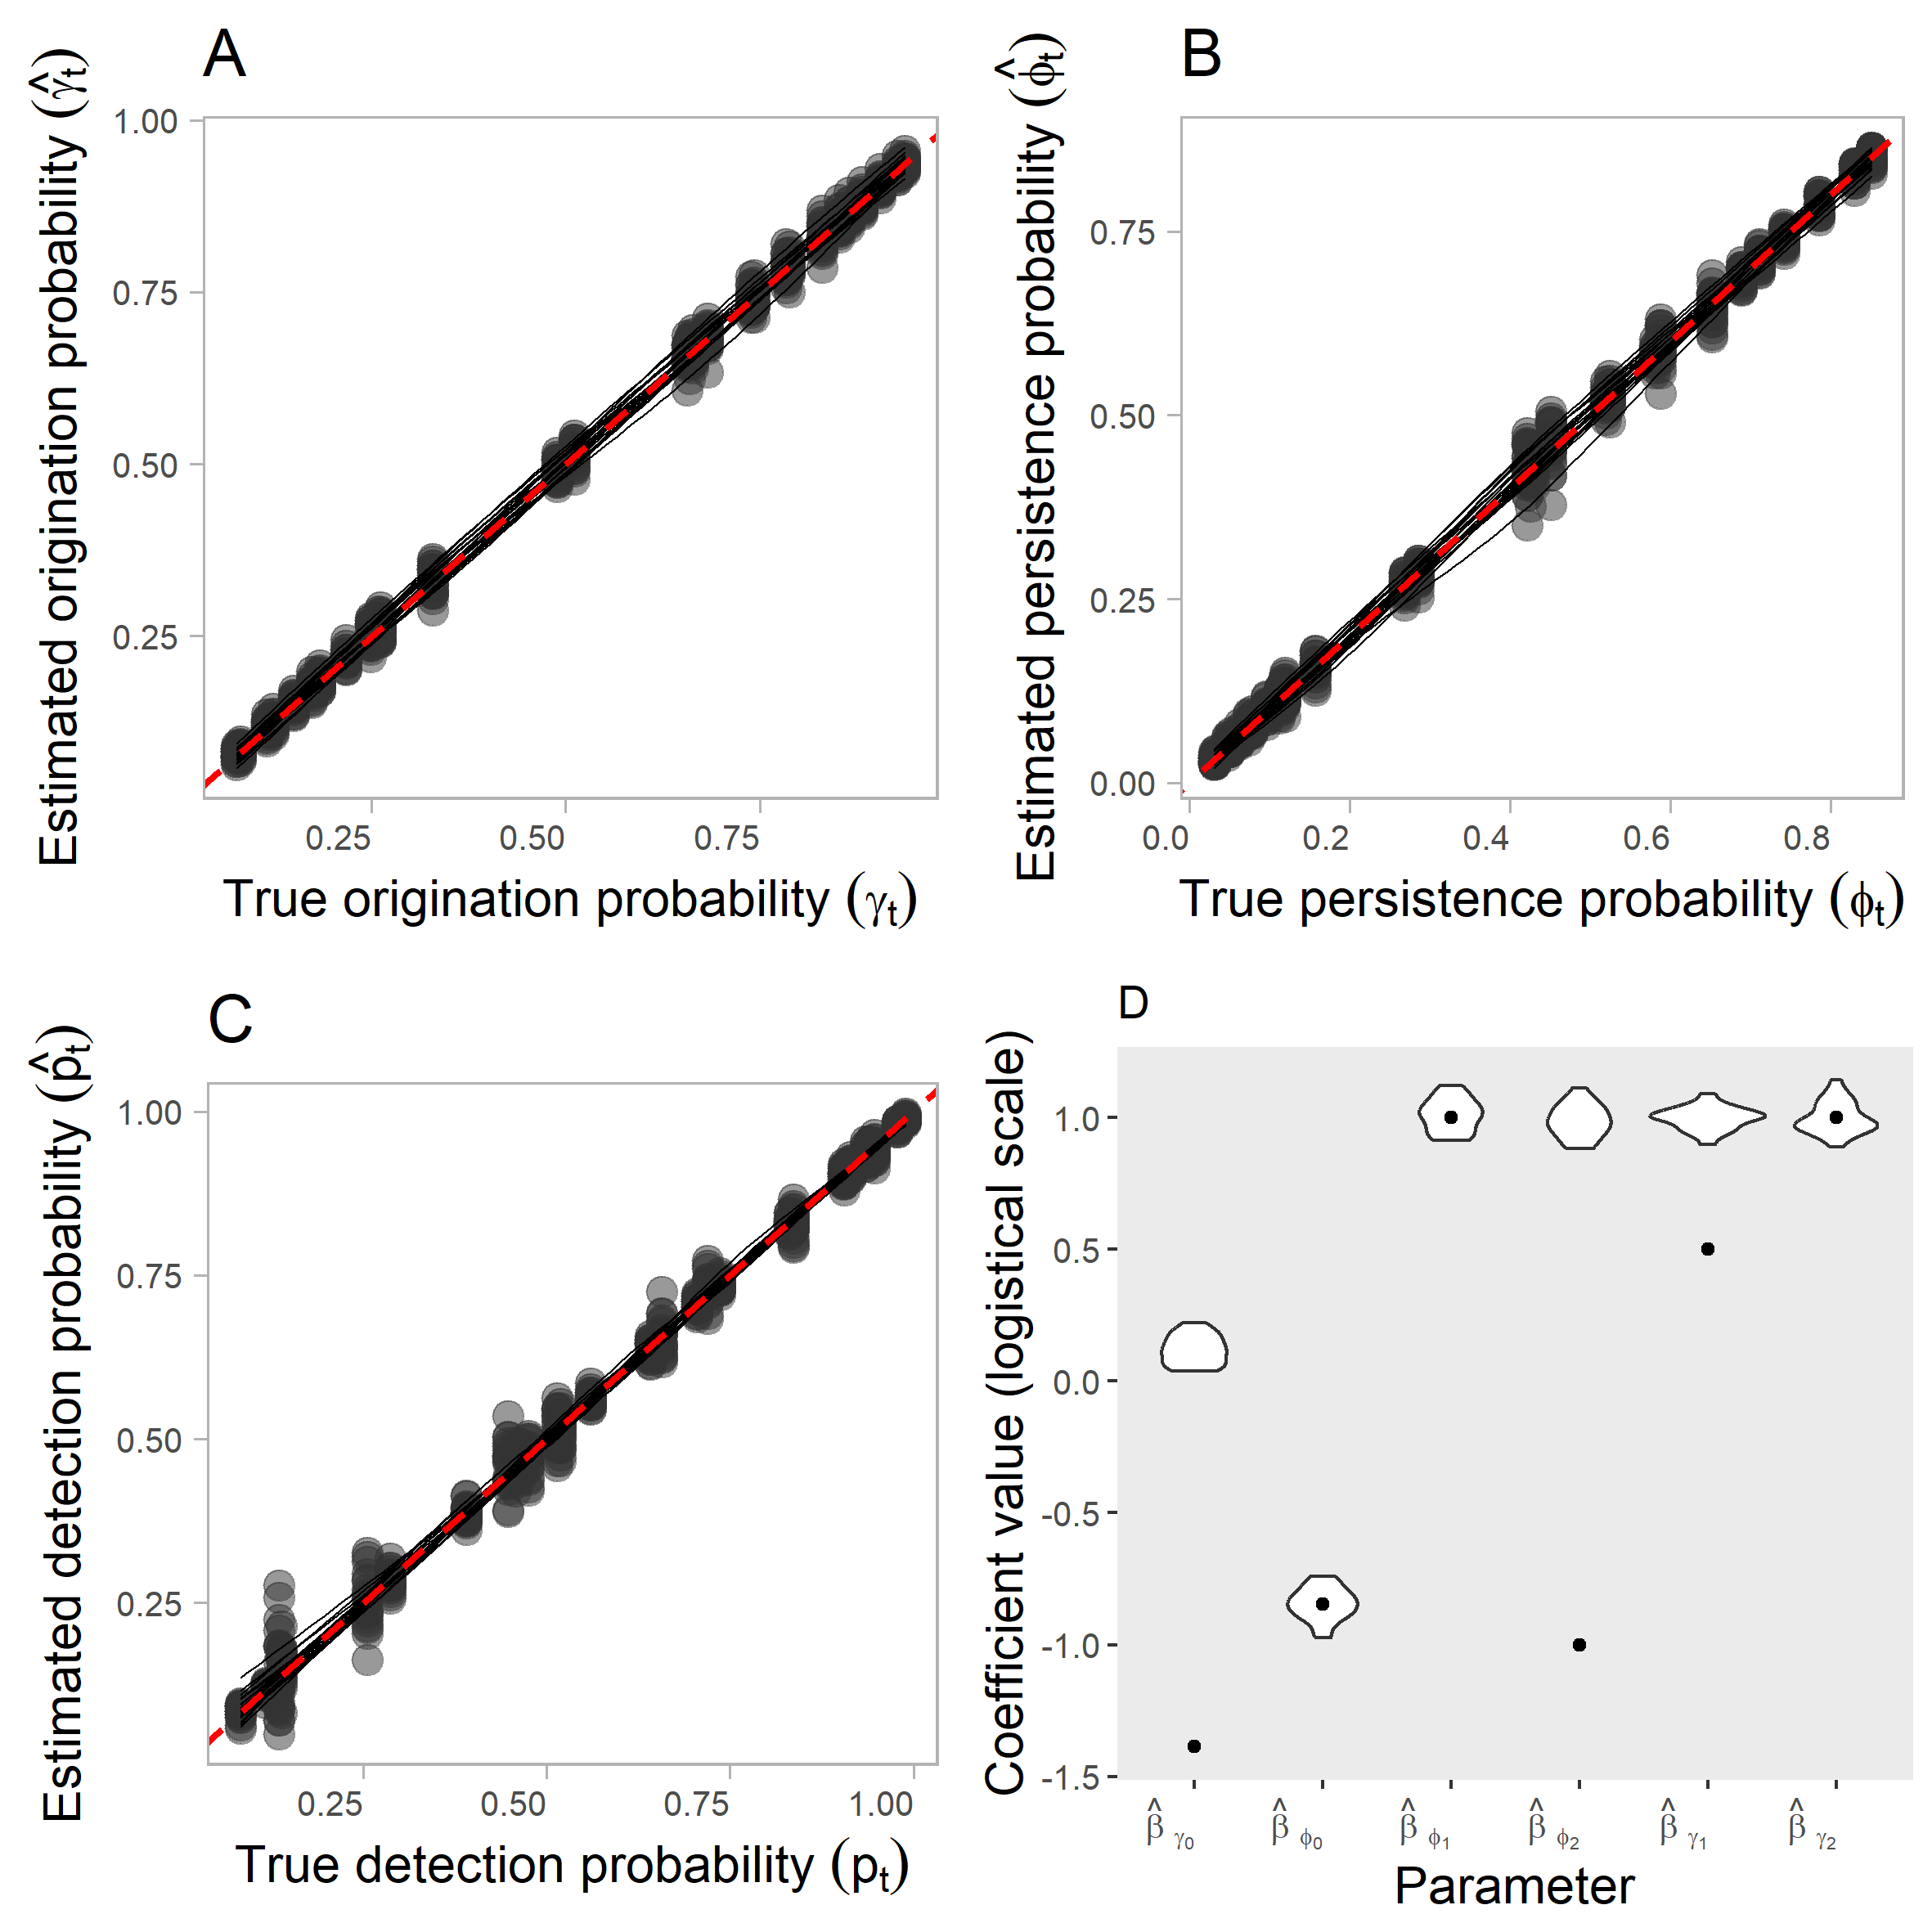
\includegraphics[width=0.75\linewidth,height=0.75\textheight]{figs/sc1} \end{center}

Fig. 1: Results depicting the performance of the model front to the
total overlap of covariates. In (A), we show the true values of
\(\gamma_t\) per time bin in the X axis, and the estimated values in the
Y axis. In (B), we show the true values of \(\phi_t\) per time bin in
the X axis, and the estimated values in the Y axis.In (C), we show the
true values of \(\p_t\) per time bin in the X axis, and the estimated
values in the Y axis. In A-C, the red line depicts the 1:1 relationship
of a perfect matching between the truth and the estimated values. One
truth-estimate relationship is shown per simulated data set (n=20). In
(D), we show violin plots (produced by the 20 simulated data setes) of
the intercepts and regression coefficients. The black points depict the
true values.

\begin{center}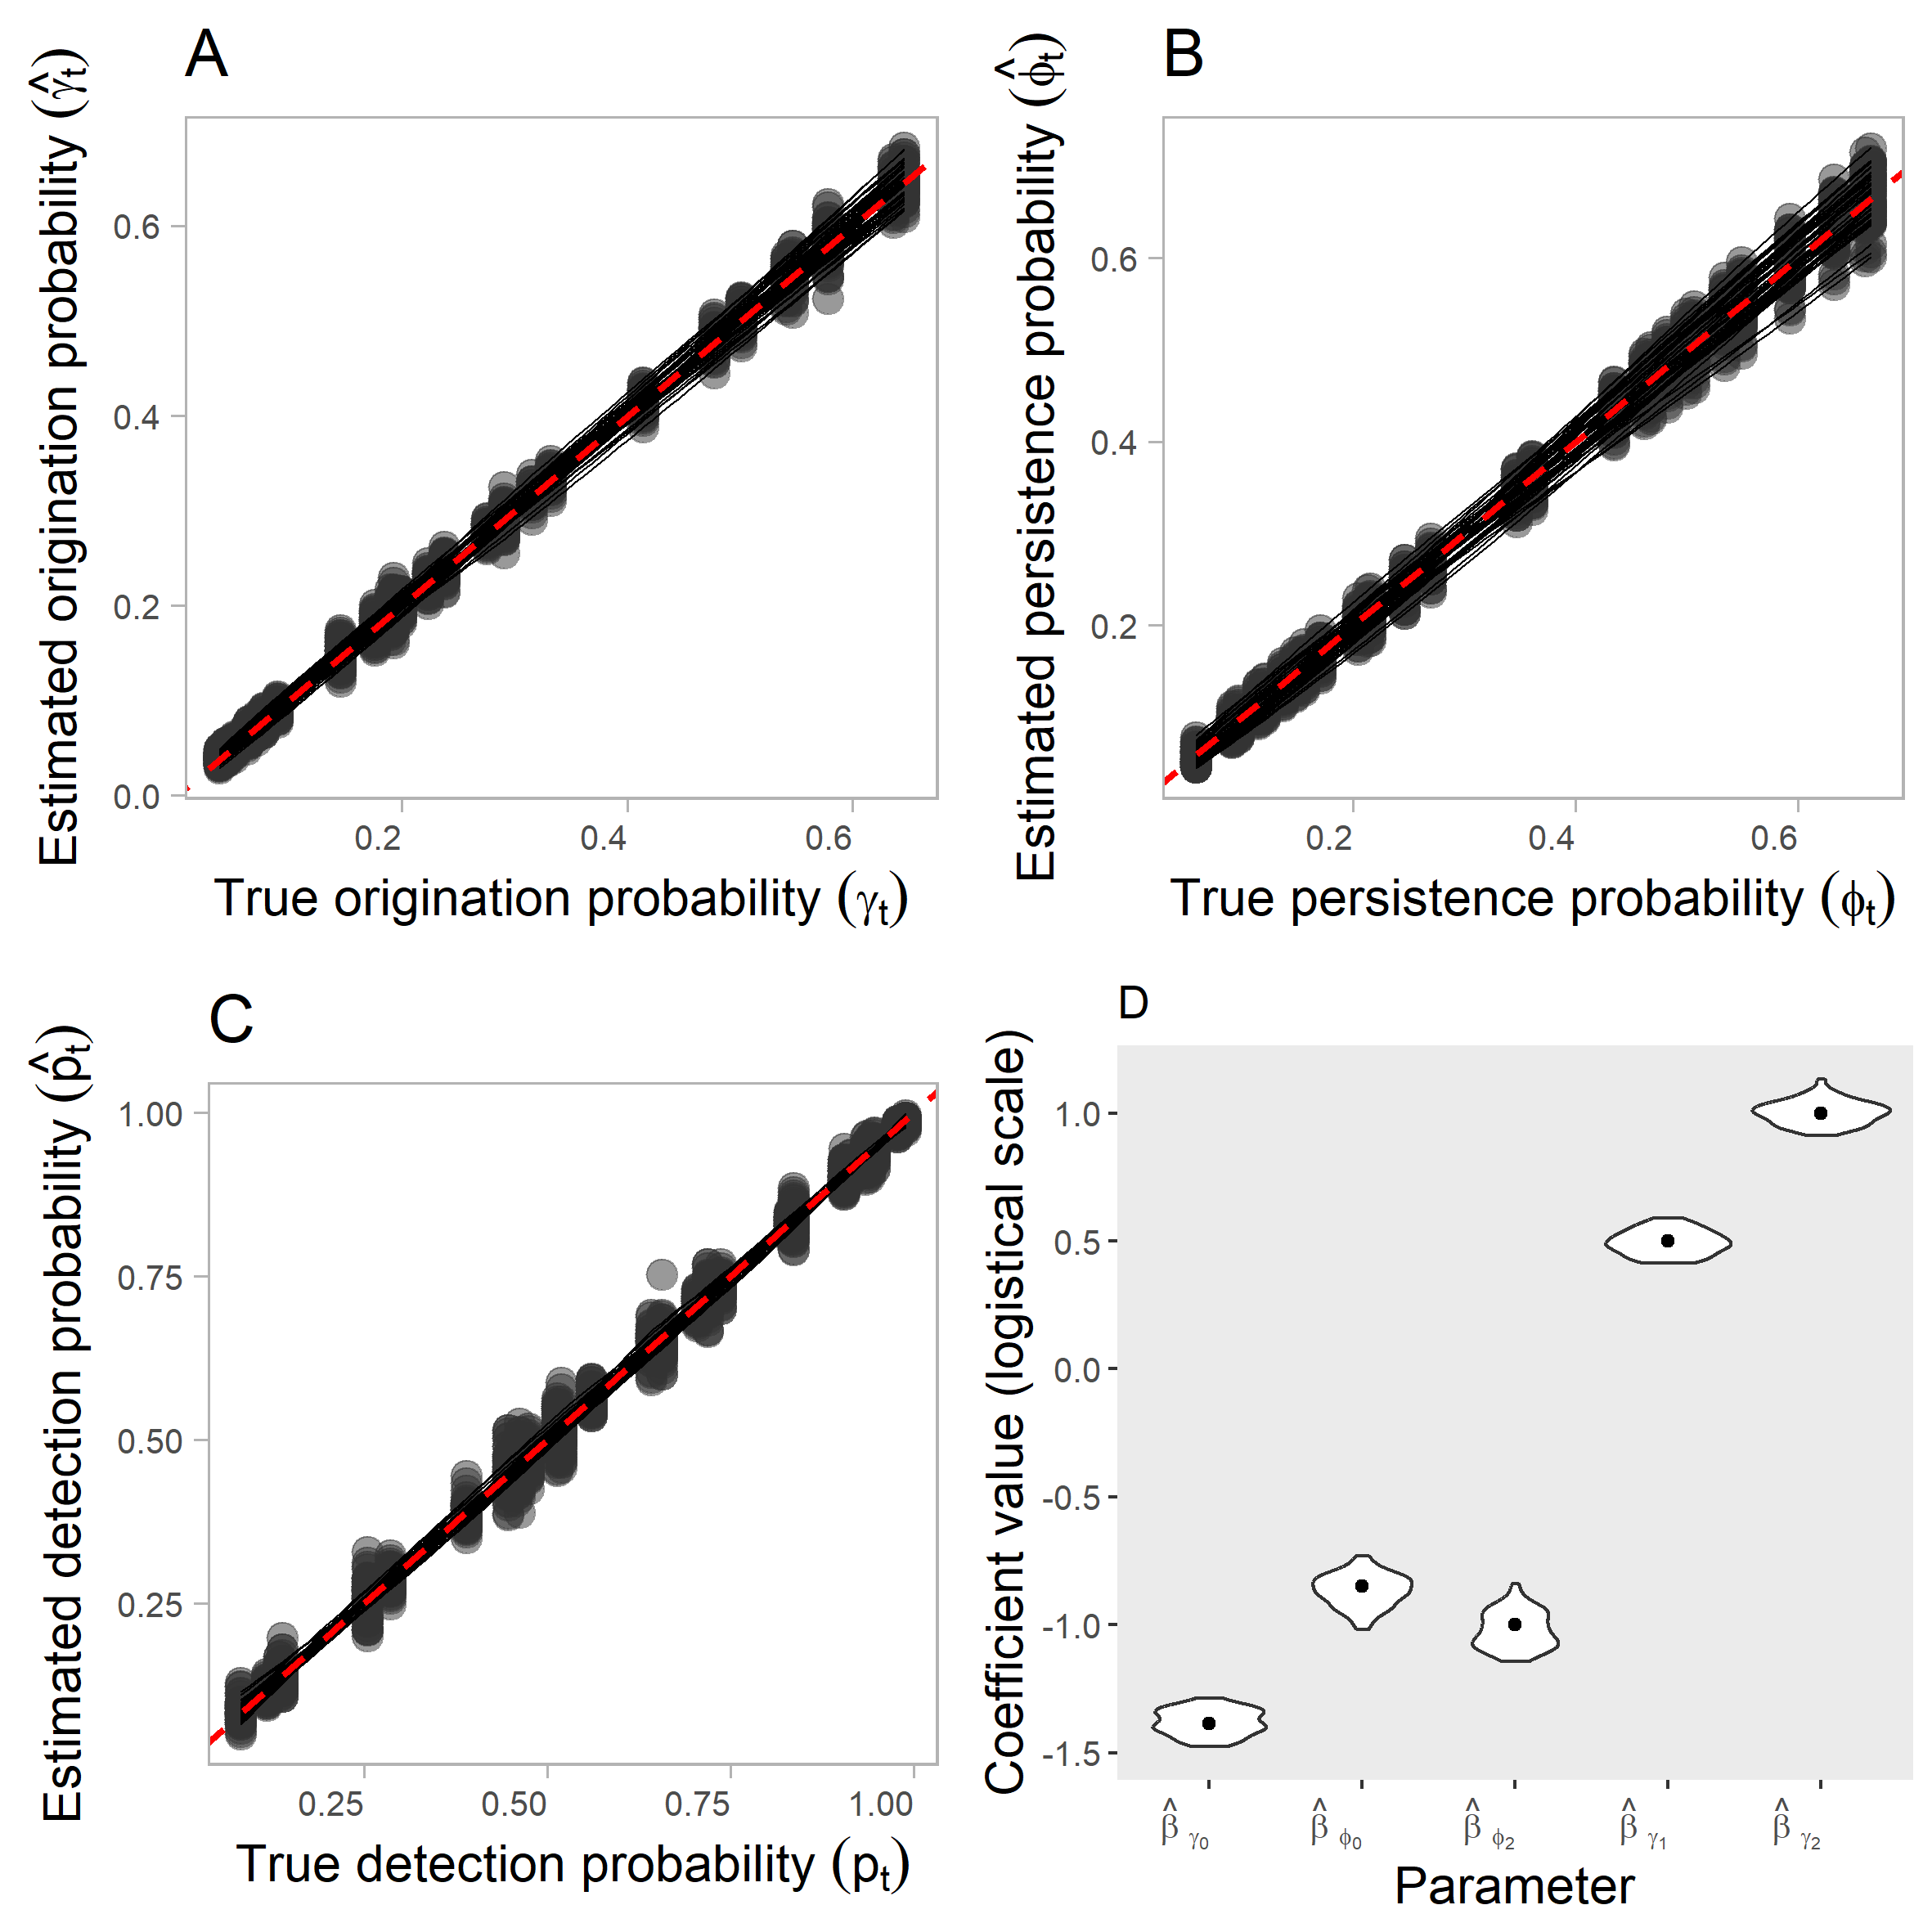
\includegraphics[width=0.75\linewidth,height=0.75\textheight]{figs/sc2} \end{center}

Fig. 2: Results depicting the performance of the model front to the
partial overlap of covariates. In (A), we show the true values of
\(\gamma_t\) per time bin in the X axis, and the estimated values in the
Y axis. In (B), we show the true values of \(\phi_t\) per time bin in
the X axis, and the estimated values in the Y axis.In (C), we show the
true values of \(\p_t\) per time bin in the X axis, and the estimated
values in the Y axis. In A-C, the red line depicts the 1:1 relationship
of a perfect matching between the truth and the estimated values. One
truth-estimate relationship is shown per simulated data set (n=20). In
(D), we show violin plots (produced by the 20 simulated data setes) of
the intercepts and regression coefficients. The black points depict the
true values.

\begin{center}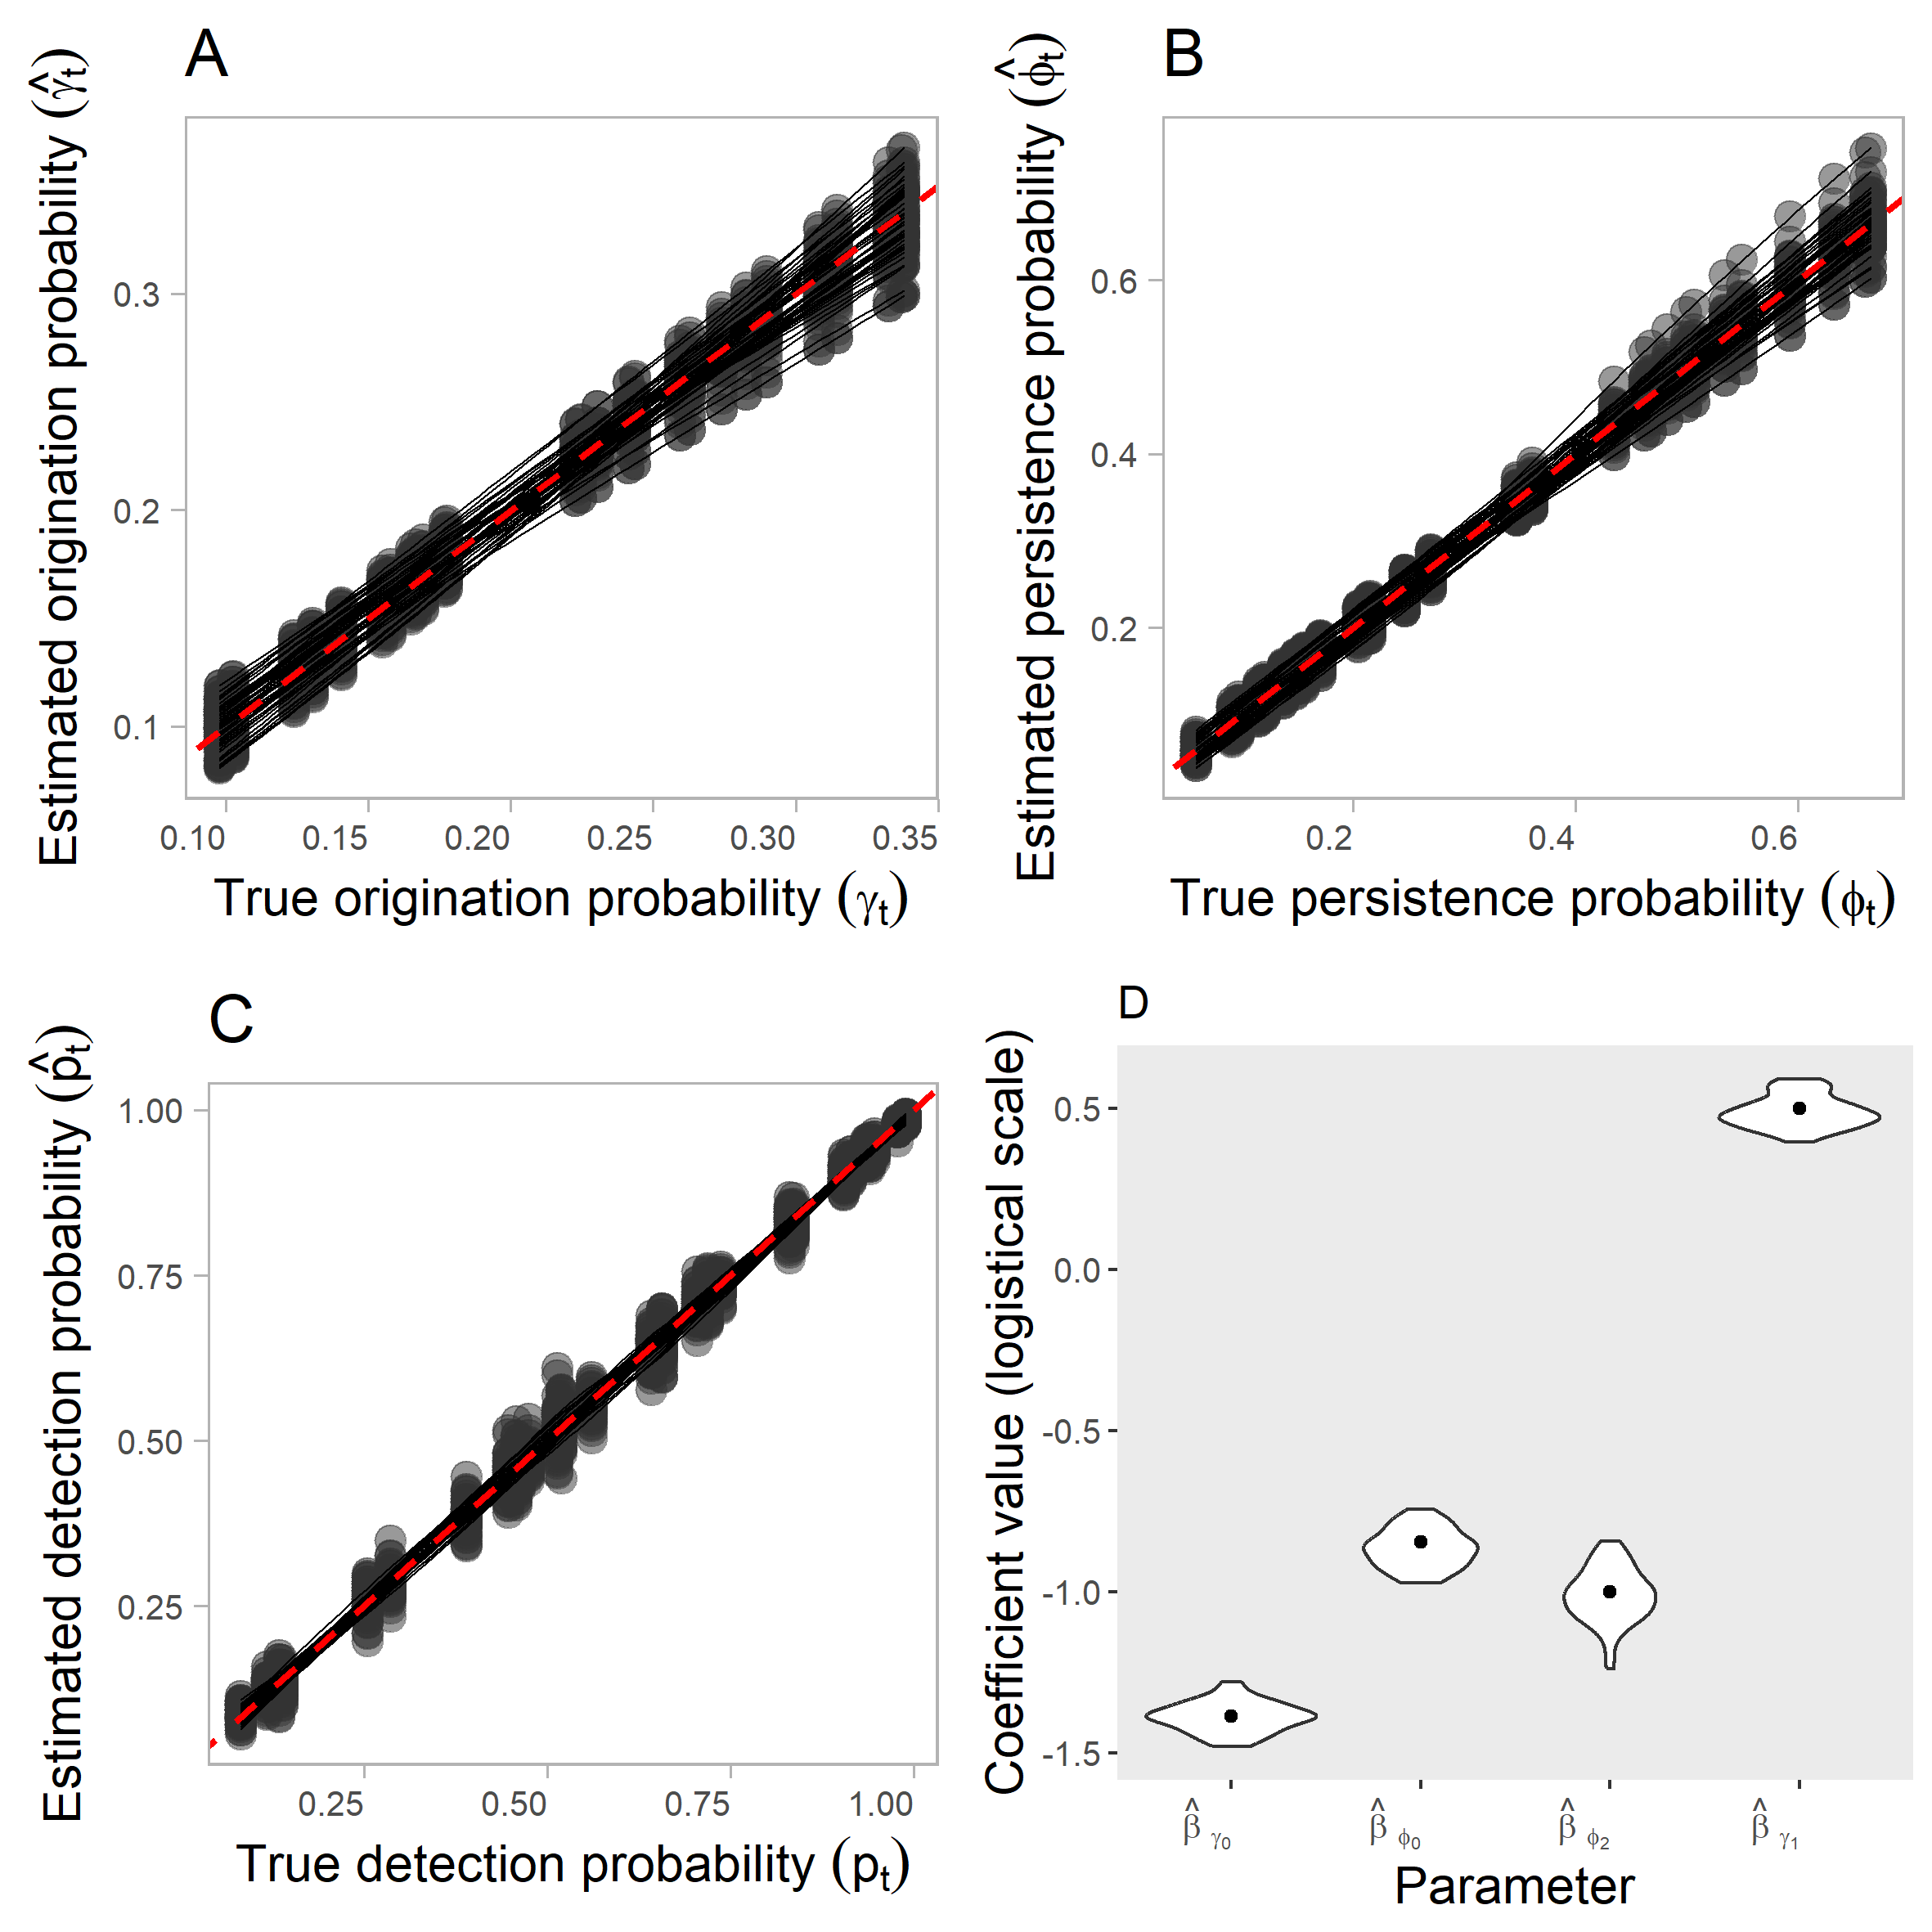
\includegraphics[width=0.75\linewidth,height=0.75\textheight]{figs/sc3} \end{center}

Fig. 3: Results depicting the performance of the model front to no
overlap of covariates. In (A), we show the true values of \(\gamma_t\)
per time bin in the X axis, and the estimated values in the Y axis. In
(B), we show the true values of \(\phi_t\) per time bin in the X axis,
and the estimated values in the Y axis.In (C), we show the true values
of \(\p_t\) per time bin in the X axis, and the estimated values in the
Y axis. In A-C, the red line depicts the 1:1 relationship of a perfect
matching between the truth and the estimated values. One truth-estimate
relationship is shown per simulated data set (n=20). In (D), we show
violin plots (produced by the 20 simulated data setes) of the intercepts
and regression coefficients. The black points depict the true values.

\hypertarget{you-can-reproduce-the-first-simulation-study-using}{%
\subsection{You can reproduce the first simulation study
using:}\label{you-can-reproduce-the-first-simulation-study-using}}

\begin{Shaded}
\begin{Highlighting}[]
\CommentTok{\# {-}{-}{-}{-}{-}{-}{-}{-}{-}{-}{-}{-}{-}{-}{-}{-}{-}{-}{-}{-}{-}{-}{-}{-}{-}{-}{-}{-}{-}{-}{-}{-}{-}{-}{-}{-}{-}{-}{-}{-}}


\CommentTok{\# Simulation study}

\CommentTok{\# Can the same set of covarites be included in the origination and extinction models??}
\CommentTok{\# global {-} scale analysis ( so the genera are in the rows of the detection table )}

\CommentTok{\# total overlap of covariates }

\CommentTok{\# {-}{-}{-}{-}{-}{-}{-}{-}{-}{-}{-}{-}{-}{-}{-}{-}{-}{-}{-}{-}{-}{-}{-}{-}{-}{-}{-}{-}{-}{-}{-}{-}{-}{-}{-}{-}{-}{-}{-}{-}}
\FunctionTok{rm}\NormalTok{(}\AttributeTok{list=}\FunctionTok{ls}\NormalTok{())}
\FunctionTok{require}\NormalTok{(here)}
\CommentTok{\# create dir}
\FunctionTok{dir.create}\NormalTok{ (}\FunctionTok{here}\NormalTok{ (}\StringTok{"simulations"}\NormalTok{, }\StringTok{"output"}\NormalTok{))}

\CommentTok{\# Write the JAGS model}
\NormalTok{model\_string }\OtherTok{\textless{}{-}} \StringTok{"}
\StringTok{model \{}
\StringTok{  }
\StringTok{      \#  Occupancy Dynamics (Priors)}
\StringTok{       }
\StringTok{       }
\StringTok{        \# {-}{-}{-}{-}{-}{-}{-}{-}{-}{-}{-}{-}{-}{-}{-}{-}{-}{-}{-}{-}{-}{-}}
\StringTok{        \#     Gamma (origination)}
\StringTok{        \# {-}{-}{-}{-}{-}{-}{-}{-}{-}{-}{-}{-}{-}{-}{-}{-}{-}{-}{-}{-}{-}{-}}
\StringTok{        }
\StringTok{        \# intercepts}
\StringTok{        gamma.u \textasciitilde{} dunif(0,1) \# range origination}
\StringTok{        intercept.gamma \textless{}{-} logit(gamma.u) \# intercept origination}
\StringTok{        }
\StringTok{        \# regression coeff}
\StringTok{        beta\_gamma1 \textasciitilde{} dunif({-}20,20)}
\StringTok{        beta\_gamma2 \textasciitilde{} dunif({-}20,20)}
\StringTok{        }
\StringTok{        \# {-}{-}{-}{-}{-}{-}{-}{-}{-}{-}{-}{-}{-}{-}{-}{-}{-}{-}{-}{-}{-}{-}}
\StringTok{        \#     Phi (persistence)}
\StringTok{        \# {-}{-}{-}{-}{-}{-}{-}{-}{-}{-}{-}{-}{-}{-}{-}{-}{-}{-}{-}{-}{-}{-}}
\StringTok{        \# intercepts}
\StringTok{        phi.u \textasciitilde{} dunif(0,1) \# range persistence}
\StringTok{        intercept.phi \textless{}{-} logit(phi.u) \# intercept persistence}
\StringTok{        }
\StringTok{        \# regression coeff}
\StringTok{        beta\_phi1 \textasciitilde{} dunif({-}20,20)}
\StringTok{        beta\_phi2 \textasciitilde{} dunif({-}20,20)}
\StringTok{       }
\StringTok{        \#\# set initial conditions for occupancy of each genus}
\StringTok{        initial\_psi \textasciitilde{} dunif(0,1)}
\StringTok{      }
\StringTok{       \#\#\#\#\#\#\#\#\#\#\#\#      Model       \#\#\#\#\#\#\#\#\#\#\#\#\#}
\StringTok{       }
\StringTok{       \# model for phi and gamma}
\StringTok{       \#\#\# model dynamic parameters}
\StringTok{        }
\StringTok{        for (t in 1:(n\_bins{-}1))\{}
\StringTok{      }
\StringTok{             \# speciation}
\StringTok{             logit(gamma[t]) \textless{}{-}  intercept.gamma + }
\StringTok{                                   beta\_gamma1*X1[t]+}
\StringTok{                                   beta\_gamma2*X2[t]}
\StringTok{                                   }
\StringTok{              \# persistence}
\StringTok{              logit(phi[t]) \textless{}{-}  intercept.phi + }
\StringTok{                                  beta\_phi1*X1[t]+}
\StringTok{                                  beta\_phi2*X2[t]}
\StringTok{                                  }
\StringTok{                                  }
\StringTok{        \}}
\StringTok{        }
\StringTok{        \# Occupancy dynamics {-}{-}{-}{-}{-}{-}{-}{-}{-}{-}{-}{-}{-}{-}{-}{-}{-}{-}{-}{-}{-}}
\StringTok{       }
\StringTok{        for (g in 1:n\_spp) \{}
\StringTok{         }
\StringTok{            z[g,1]\textasciitilde{}dbern(initial\_psi) \# occupancy status initialization}
\StringTok{      }
\StringTok{                for (t in 2:n\_bins)\{}
\StringTok{              }
\StringTok{                  \# model likelihood}
\StringTok{                  \#\#\# modeling dynamics conditional on previous time realized occurrence z}
\StringTok{                  muZ[g,t] \textless{}{-} z[g,t{-}1] *  phi[t{-}1] + \#\#\# if occupied, p of not getting extinct/persist in the next time}
\StringTok{                                (1{-}z[g,t{-}1]) *  gamma[t{-}1] \#\#\#  if not occupied, p of originate in the next time}
\StringTok{                  }
\StringTok{                 \# realized occurrence}
\StringTok{                 muZW[g,t] \textless{}{-} muZ[g,t]}
\StringTok{                   z[g,t] \textasciitilde{} dbern(muZW[g,t])}
\StringTok{              }
\StringTok{          \}\#t}
\StringTok{        }
\StringTok{        \} \#g}
\StringTok{  }
\StringTok{  }
\StringTok{    \#\#\#\#\#\#\#\#\#\#\#\#\#\#\#\#\#\#\#\#\#\#\#\#\#\#\#\#\#\#\#\#\#\#\#\#\#\#\#\#\#\#\#\#\#\#\#\#\#\#\#\#\#\#\#\#\#\#\#\#\#}
\StringTok{    \#                                                           \#}
\StringTok{    \#         Observation process across formations             \#}
\StringTok{    \#                                                           \#}
\StringTok{    \#\#\#\#\#\#\#\#\#\#\#\#\#\#\#\#\#\#\#\#\#\#\#\#\#\#\#\#\#\#\#\#\#\#\#\#\#\#\#\#\#\#\#\#\#\#\#\#\#\#\#\#\#\#\#\#\#\#\#\#\#}
\StringTok{    }
\StringTok{    \#\#\#  detection intercept}
\StringTok{    \# intercept    }
\StringTok{    for (t in 1:n\_bins) \{}
\StringTok{      p[t] \textasciitilde{} dunif(0,1) }
\StringTok{    \}}
\StringTok{    }
\StringTok{    \# observation submodel}
\StringTok{    for (g in 1:n\_spp) \{ \#\# loop over genera }
\StringTok{      }
\StringTok{      for (t in 1:n\_bins) \{ \#\# loop over time bins }
\StringTok{    }
\StringTok{          \# observation}
\StringTok{          \# Specify the binomial observation model conditional on occupancy state}
\StringTok{          y[g,t] \textasciitilde{} dbin(muY[g,t], n\_surveys[t])}
\StringTok{          muY[g,t] \textless{}{-} z[g,t]*p[t]}
\StringTok{                  }
\StringTok{        \}}
\StringTok{      }
\StringTok{    \}}
\StringTok{      }

\StringTok{\}}

\StringTok{"}

\CommentTok{\# Load necessary libraries}
\FunctionTok{library}\NormalTok{(jagsUI)}
\FunctionTok{library}\NormalTok{(here)}

\CommentTok{\# Set parameters}
\FunctionTok{set.seed}\NormalTok{(}\DecValTok{42}\NormalTok{)}
\NormalTok{n\_spp }\OtherTok{\textless{}{-}} \DecValTok{200}  \CommentTok{\# Number of genera}
\NormalTok{n\_bins }\OtherTok{\textless{}{-}} \DecValTok{30}   \CommentTok{\# Number of time bins}
\NormalTok{n\_surveys }\OtherTok{\textless{}{-}} \DecValTok{10}  \CommentTok{\# Number of surveys (geological formations) per time bin}

\CommentTok{\# Initial occupancy probability}
\NormalTok{initial\_psi }\OtherTok{\textless{}{-}} \FloatTok{0.3}

\CommentTok{\# Detection probability}
\NormalTok{p }\OtherTok{\textless{}{-}} \FunctionTok{runif}\NormalTok{(n\_bins,}\DecValTok{0}\NormalTok{,}\DecValTok{1}\NormalTok{)  }

\CommentTok{\# covariate effect on origination}
\NormalTok{intercept\_gamma }\OtherTok{\textless{}{-}} \FunctionTok{qlogis}\NormalTok{(}\FloatTok{0.2}\NormalTok{) }
\NormalTok{beta\_gamma1 }\OtherTok{\textless{}{-}} \FloatTok{0.5}
\NormalTok{beta\_gamma2 }\OtherTok{\textless{}{-}} \DecValTok{1}

\CommentTok{\# covariate effect on persistence}
\NormalTok{intercept\_phi }\OtherTok{\textless{}{-}} \FunctionTok{qlogis}\NormalTok{(}\FloatTok{0.3}\NormalTok{)  }
\NormalTok{beta\_phi1 }\OtherTok{\textless{}{-}} \DecValTok{1}
\NormalTok{beta\_phi2 }\OtherTok{\textless{}{-}} \SpecialCharTok{{-}}\DecValTok{1}

\CommentTok{\# covariates (generate just once and save to be used in the other two simulation sets)}
\NormalTok{X1 }\OtherTok{\textless{}{-}} \FunctionTok{runif}\NormalTok{ (n\_bins}\DecValTok{{-}1}\NormalTok{, }\SpecialCharTok{{-}}\DecValTok{2}\NormalTok{, }\DecValTok{2}\NormalTok{) }
\NormalTok{X2 }\OtherTok{\textless{}{-}} \FunctionTok{runif}\NormalTok{ (n\_bins}\DecValTok{{-}1}\NormalTok{, }\SpecialCharTok{{-}}\DecValTok{2}\NormalTok{, }\DecValTok{2}\NormalTok{)  }
\FunctionTok{save}\NormalTok{(X1,X2, }\AttributeTok{file=}\FunctionTok{here}\NormalTok{(}\StringTok{"simulations"}\NormalTok{,}\StringTok{"covariates.RData"}\NormalTok{))}
\CommentTok{\# load(file=here("simulations","covariates.RData")) \# activate after the creation}
\FunctionTok{cor}\NormalTok{(}\FunctionTok{cbind}\NormalTok{(X1,X2))}

\CommentTok{\# scale covariates}
\NormalTok{X1}\OtherTok{\textless{}{-}}\FunctionTok{scale}\NormalTok{(X1)[,}\DecValTok{1}\NormalTok{]}
\NormalTok{X2}\OtherTok{\textless{}{-}}\FunctionTok{scale}\NormalTok{(X2)[,}\DecValTok{1}\NormalTok{]}


\CommentTok{\# start simulations {-}{-}{-}{-}{-}{-}{-}{-}{-}{-}{-}{-}{-}{-}{-}{-}{-}{-}{-}{-}{-}{-}{-}{-}{-}{-}{-}{-}{-}{-}{-}{-}{-}}

\NormalTok{n.sims }\OtherTok{\textless{}{-}} \DecValTok{20}
\NormalTok{my.seeds }\OtherTok{\textless{}{-}} \FunctionTok{floor}\NormalTok{(}\FunctionTok{runif}\NormalTok{ (n.sims,}\DecValTok{0}\NormalTok{,}\DecValTok{5000}\NormalTok{))}

\CommentTok{\# run}
\FunctionTok{lapply}\NormalTok{ (}\FunctionTok{seq}\NormalTok{(}\DecValTok{1}\NormalTok{,n.sims), }\ControlFlowTok{function}\NormalTok{ (s) \{}
  
        \CommentTok{\# set seed}
        \FunctionTok{set.seed}\NormalTok{(my.seeds[s])}
        
        \CommentTok{\# Origination probability}
\NormalTok{        phi }\OtherTok{\textless{}{-}}\NormalTok{ gamma }\OtherTok{\textless{}{-}} \FunctionTok{array}\NormalTok{(}\ConstantTok{NA}\NormalTok{, }\AttributeTok{dim =}\NormalTok{ (n\_bins}\DecValTok{{-}1}\NormalTok{)) }\CommentTok{\# persistence, colonisation}
         
        \CommentTok{\# produce transition probs}
        \ControlFlowTok{for}\NormalTok{(t }\ControlFlowTok{in} \DecValTok{1}\SpecialCharTok{:}\NormalTok{(n\_bins}\DecValTok{{-}1}\NormalTok{))\{}
          
            \CommentTok{\# origination }
\NormalTok{            gamma[t] }\OtherTok{\textless{}{-}} \FunctionTok{plogis}\NormalTok{(intercept\_gamma}\SpecialCharTok{+}\NormalTok{beta\_gamma1}\SpecialCharTok{+}\NormalTok{X1[t]}\SpecialCharTok{+}
\NormalTok{                                      beta\_gamma2}\SpecialCharTok{+}\NormalTok{X2[t])}
            
            \CommentTok{\# persistence probability}
\NormalTok{            phi[t] }\OtherTok{\textless{}{-}} \FunctionTok{plogis}\NormalTok{(intercept\_phi}\SpecialCharTok{+}\NormalTok{beta\_phi1}\SpecialCharTok{+}\NormalTok{X1[t]}\SpecialCharTok{+}
\NormalTok{                                    beta\_phi2}\SpecialCharTok{+}\NormalTok{X2[t])}\CommentTok{\# back to prob scale}
            
            
\NormalTok{        \}}
        
        \CommentTok{\# Simulate occupancy states}
\NormalTok{        z }\OtherTok{\textless{}{-}} \FunctionTok{array}\NormalTok{(}\ConstantTok{NA}\NormalTok{, }\AttributeTok{dim =} \FunctionTok{c}\NormalTok{(n\_spp, n\_bins))}
\NormalTok{        muZ }\OtherTok{\textless{}{-}} \FunctionTok{array}\NormalTok{(}\ConstantTok{NA}\NormalTok{, }\AttributeTok{dim =} \FunctionTok{c}\NormalTok{(n\_spp, n\_bins))}
\NormalTok{        z[, }\DecValTok{1}\NormalTok{] }\OtherTok{\textless{}{-}} \FunctionTok{rbinom}\NormalTok{(n\_spp, }\DecValTok{1}\NormalTok{, initial\_psi)}
        
        \CommentTok{\# true incidence}
        \ControlFlowTok{for}\NormalTok{ (i }\ControlFlowTok{in} \DecValTok{1}\SpecialCharTok{:}\NormalTok{n\_spp) \{}
            \ControlFlowTok{for}\NormalTok{ (t }\ControlFlowTok{in} \DecValTok{2}\SpecialCharTok{:}\NormalTok{n\_bins) \{}
\NormalTok{              muZ[i,t] }\OtherTok{\textless{}{-}}\NormalTok{ z[i, t }\SpecialCharTok{{-}} \DecValTok{1}\NormalTok{] }\SpecialCharTok{*}\NormalTok{ phi[t}\DecValTok{{-}1}\NormalTok{] }\SpecialCharTok{+}\NormalTok{ (}\DecValTok{1} \SpecialCharTok{{-}}\NormalTok{ z[i, t }\SpecialCharTok{{-}} \DecValTok{1}\NormalTok{]) }\SpecialCharTok{*}\NormalTok{ gamma[t}\DecValTok{{-}1}\NormalTok{]}
\NormalTok{              z[i, t] }\OtherTok{\textless{}{-}} \FunctionTok{rbinom}\NormalTok{(}\DecValTok{1}\NormalTok{, }\DecValTok{1}\NormalTok{, muZ[i,t])}
\NormalTok{          \}}
\NormalTok{        \}}
        
        \CommentTok{\# Simulate detections}
\NormalTok{        y }\OtherTok{\textless{}{-}} \FunctionTok{array}\NormalTok{(}\ConstantTok{NA}\NormalTok{, }\AttributeTok{dim =} \FunctionTok{c}\NormalTok{(n\_spp, n\_bins))}
        \ControlFlowTok{for}\NormalTok{ (i }\ControlFlowTok{in} \DecValTok{1}\SpecialCharTok{:}\NormalTok{n\_spp) \{}
          \ControlFlowTok{for}\NormalTok{ (t }\ControlFlowTok{in} \DecValTok{1}\SpecialCharTok{:}\NormalTok{n\_bins) \{}
            
\NormalTok{              y[i, t] }\OtherTok{\textless{}{-}} \FunctionTok{rbinom}\NormalTok{(}\DecValTok{1}\NormalTok{, }\FunctionTok{rep}\NormalTok{(n\_surveys,n\_bins), z[i, t] }\SpecialCharTok{*}\NormalTok{ p[t])}
            
\NormalTok{          \}}
\NormalTok{        \}}
        
        \CommentTok{\#save data}
        \FunctionTok{save}\NormalTok{ (y,z ,muZ,p, phi,gamma, }\AttributeTok{file =} \FunctionTok{here}\NormalTok{ (}\StringTok{"simulations"}\NormalTok{, }\StringTok{"output"}\NormalTok{, }\FunctionTok{paste0}\NormalTok{(}\StringTok{"data\_"}\NormalTok{, s,}\StringTok{".RData"}\NormalTok{)))}
        
        \CommentTok{\# Prepare data for JAGS}
\NormalTok{        jags\_data }\OtherTok{\textless{}{-}} \FunctionTok{list}\NormalTok{(}
          \AttributeTok{y =}\NormalTok{ y,}
          \AttributeTok{n\_spp =}\NormalTok{ n\_spp,}
          \AttributeTok{n\_bins =}\NormalTok{ n\_bins,}
          \AttributeTok{n\_surveys =} \FunctionTok{rep}\NormalTok{(n\_surveys,n\_bins),}
          \AttributeTok{X1=}\NormalTok{X1,}
          \AttributeTok{X2=}\NormalTok{X2}
\NormalTok{        )}
        
        \CommentTok{\# Initial values for the latent states}
\NormalTok{        init\_values }\OtherTok{\textless{}{-}} \ControlFlowTok{function}\NormalTok{() \{}
          \FunctionTok{list}\NormalTok{(}\AttributeTok{z =} \FunctionTok{ifelse}\NormalTok{(y}\SpecialCharTok{\textgreater{}}\DecValTok{0}\NormalTok{,}\DecValTok{1}\NormalTok{,}\DecValTok{0}\NormalTok{),}
               \AttributeTok{phi.u =} \FloatTok{0.3}\NormalTok{,}
               \AttributeTok{gamma.u=}\FloatTok{0.2}
               
\NormalTok{               )}
\NormalTok{        \}}
        
        \CommentTok{\# Parameters to monitor}
\NormalTok{        parameters }\OtherTok{\textless{}{-}} \FunctionTok{c}\NormalTok{(}\StringTok{"intercept.phi"}\NormalTok{,}
                        \StringTok{"beta\_phi1"}\NormalTok{,}
                        \StringTok{"beta\_phi2"}\NormalTok{,}
                        \StringTok{"intercept.gamma"}\NormalTok{,}
                        \StringTok{"beta\_gamma1"}\NormalTok{,}
                        \StringTok{"beta\_gamma2"}\NormalTok{,}
                        \StringTok{"initial\_psi"}\NormalTok{, }
                        \StringTok{"gamma"}\NormalTok{,}
                        \StringTok{"phi"}\NormalTok{,}
                        \StringTok{"p"}\NormalTok{, }
                        \StringTok{"muZ"}\NormalTok{)}
        
        \CommentTok{\# Run JAGS model}
        \DocumentationTok{\#\# MCMC runs}
\NormalTok{        samples }\OtherTok{\textless{}{-}}\FunctionTok{jags}\NormalTok{ (}\AttributeTok{data =}\NormalTok{ jags\_data, }
                        \AttributeTok{parameters.to.save =}\NormalTok{ parameters, }
                        \AttributeTok{model.file =} \FunctionTok{textConnection}\NormalTok{(model\_string), }
                        \AttributeTok{inits =}\NormalTok{ init\_values, }
                        \AttributeTok{n.chains =} \DecValTok{3}\NormalTok{, }
                        \AttributeTok{n.thin =} \DecValTok{1}\NormalTok{, }
                        \AttributeTok{n.iter =} \DecValTok{500}\NormalTok{,}
                        \AttributeTok{n.adapt =} \DecValTok{200}\NormalTok{,}
                        \AttributeTok{n.burnin =} \DecValTok{400}\NormalTok{, }
                        \AttributeTok{DIC =}\NormalTok{ T,  }
                        \AttributeTok{parallel=}\NormalTok{F}
\NormalTok{        )}
        
        \CommentTok{\# extract summary}
\NormalTok{        point\_estimates }\OtherTok{\textless{}{-}}\NormalTok{ samples}\SpecialCharTok{$}\NormalTok{summary}
        
        \CommentTok{\#save}
        \FunctionTok{save}\NormalTok{ (point\_estimates, }\AttributeTok{file =} \FunctionTok{here}\NormalTok{ (}\StringTok{"simulations"}\NormalTok{, }\StringTok{"output"}\NormalTok{, }\FunctionTok{paste0}\NormalTok{(}\StringTok{"sims\_run"}\NormalTok{, s,}\StringTok{".RData"}\NormalTok{)))}
        
        
\NormalTok{\})}

\CommentTok{\# end}
\end{Highlighting}
\end{Shaded}

You can generate the arrange of plots using the following code:

\begin{Shaded}
\begin{Highlighting}[]
\CommentTok{\# {-}{-}{-}{-}{-}{-}{-}{-}{-}{-}{-}{-}{-}{-}{-}{-}{-}{-}{-}{-}{-}{-}{-}{-}{-}{-}{-}{-}{-}{-}{-}{-}{-}{-}{-}{-}{-}{-}{-}{-}}

\CommentTok{\# Load necessary libraries {-}{-}{-}{-}{-}{-}{-}{-}{-}{-}{-}{-}{-}{-}{-}{-}{-}{-}{-}{-}{-}{-}{-}{-}{-}{-}{-}{-}{-}{-}{-}{-}{-}{-}{-}{-}{-}{-}}
\FunctionTok{rm}\NormalTok{(}\AttributeTok{list=}\FunctionTok{ls}\NormalTok{())}
\FunctionTok{library}\NormalTok{(rjags)}
\FunctionTok{library}\NormalTok{(here)}

\CommentTok{\# create dir}
\FunctionTok{dir.create}\NormalTok{ (}\FunctionTok{here}\NormalTok{ (}\StringTok{"simulations"}\NormalTok{, }\StringTok{"figs"}\NormalTok{))}

\CommentTok{\# load output {-}{-}{-}{-}{-}{-}{-}{-}{-}{-}{-}{-}{-}{-}{-}{-}{-}{-}{-}{-}{-}{-}{-}{-}{-}{-}{-}{-}{-}{-}{-}{-}{-}}
\CommentTok{\# results}
\NormalTok{filenames }\OtherTok{\textless{}{-}} \FunctionTok{list.files}\NormalTok{(}\FunctionTok{here}\NormalTok{ (}\StringTok{"simulations"}\NormalTok{, }\StringTok{"output"}\NormalTok{), }\AttributeTok{full.names=}\NormalTok{T, }\AttributeTok{pattern =} \StringTok{"sims\_run"}\NormalTok{)}
\NormalTok{results }\OtherTok{\textless{}{-}} \FunctionTok{sapply}\NormalTok{(filenames, }\ControlFlowTok{function}\NormalTok{(x) }\FunctionTok{mget}\NormalTok{(}\FunctionTok{load}\NormalTok{(x)), }\AttributeTok{simplify =} \ConstantTok{TRUE}\NormalTok{)}

\CommentTok{\# simulated data}
\NormalTok{filenames }\OtherTok{\textless{}{-}} \FunctionTok{list.files}\NormalTok{(}\FunctionTok{here}\NormalTok{ (}\StringTok{"simulations"}\NormalTok{, }\StringTok{"output"}\NormalTok{), }\AttributeTok{full.names=}\NormalTok{T,}\AttributeTok{pattern =} \StringTok{"data"}\NormalTok{)}
\NormalTok{simdata }\OtherTok{\textless{}{-}} \FunctionTok{sapply}\NormalTok{(filenames, }\ControlFlowTok{function}\NormalTok{(x) }\FunctionTok{mget}\NormalTok{(}\FunctionTok{load}\NormalTok{(x)), }\AttributeTok{simplify =}\NormalTok{ F)}

\CommentTok{\# bind}
\NormalTok{df\_res }\OtherTok{\textless{}{-}} \FunctionTok{do.call}\NormalTok{(rbind,results)}

\CommentTok{\# find variables I want}
\NormalTok{hat\_gamma }\OtherTok{\textless{}{-}}\NormalTok{ df\_res [}\FunctionTok{grep}\NormalTok{(}\StringTok{"gamma"}\NormalTok{, }\FunctionTok{rownames}\NormalTok{(df\_res)),]}
\NormalTok{hat\_gamma }\OtherTok{\textless{}{-}}\NormalTok{ hat\_gamma [}\SpecialCharTok{{-}}\FunctionTok{grep}\NormalTok{(}\StringTok{"intercept"}\NormalTok{,}\FunctionTok{rownames}\NormalTok{(hat\_gamma)),] }\CommentTok{\# remove intercept}
\NormalTok{hat\_gamma }\OtherTok{\textless{}{-}}\NormalTok{ hat\_gamma [}\SpecialCharTok{{-}}\FunctionTok{grep}\NormalTok{(}\StringTok{"beta"}\NormalTok{,}\FunctionTok{rownames}\NormalTok{(hat\_gamma)),] }\CommentTok{\# remove coeffs}

\CommentTok{\# plot}
\FunctionTok{require}\NormalTok{(reshape)}
\FunctionTok{require}\NormalTok{(dplyr)}
\FunctionTok{require}\NormalTok{(ggplot2)}

\NormalTok{my\_theme }\OtherTok{\textless{}{-}} \FunctionTok{theme}\NormalTok{(}\AttributeTok{legend.position =} \StringTok{\textquotesingle{}bottom\textquotesingle{}}\NormalTok{, }
                  \AttributeTok{strip.text =} \FunctionTok{element\_text}\NormalTok{(}\AttributeTok{size=}\DecValTok{12}\NormalTok{),}
                  \AttributeTok{strip.text.y =} \FunctionTok{element\_text}\NormalTok{(}\AttributeTok{color =} \StringTok{\textquotesingle{}black\textquotesingle{}}\NormalTok{),}
                  \AttributeTok{strip.text.x =} \FunctionTok{element\_text}\NormalTok{(}\AttributeTok{color =} \StringTok{\textquotesingle{}black\textquotesingle{}}\NormalTok{), }
                  \CommentTok{\#text = element\_text(family="LM Roman 10"),}
                  \AttributeTok{panel.grid.major =} \FunctionTok{element\_blank}\NormalTok{(),}
                  \AttributeTok{panel.grid.minor =} \FunctionTok{element\_blank}\NormalTok{(),}
                  \AttributeTok{axis.text.x =} \FunctionTok{element\_text}\NormalTok{(}\AttributeTok{angle =} \DecValTok{0}\NormalTok{, }\AttributeTok{hjust =} \DecValTok{1}\NormalTok{, }\AttributeTok{size =} \DecValTok{10}\NormalTok{), }
                  \AttributeTok{axis.text.y =} \FunctionTok{element\_text}\NormalTok{(}\AttributeTok{size =} \DecValTok{10}\NormalTok{),}
                  \AttributeTok{axis.title =} \FunctionTok{element\_text}\NormalTok{(}\AttributeTok{size=}\DecValTok{15}\NormalTok{))}

\CommentTok{\# plot phi and gamma {-}{-}{-}{-}{-}{-}{-}{-}{-}{-}{-}{-}{-}{-}{-}{-}{-}{-}{-}{-}{-}{-}{-}{-}{-}{-}{-}{-}{-}{-}{-}{-}{-}{-}{-}{-}{-}{-}{-}{-}{-}{-}{-}{-}}

\NormalTok{p\_gamma}\OtherTok{\textless{}{-}}\FunctionTok{data.frame}\NormalTok{ (}\AttributeTok{hat\_gamma =} \FunctionTok{melt}\NormalTok{(}\FunctionTok{matrix}\NormalTok{(hat\_gamma[,}\StringTok{"mean"}\NormalTok{],}\AttributeTok{ncol=}\DecValTok{20}\NormalTok{,}\AttributeTok{byrow=}\NormalTok{F)),}
            \AttributeTok{true\_gamma =} \FunctionTok{melt}\NormalTok{(}\FunctionTok{sapply}\NormalTok{ (simdata, }\StringTok{"[["}\NormalTok{,}\StringTok{"gamma"}\NormalTok{ ))[,}\DecValTok{3}\NormalTok{]) }\SpecialCharTok{\%\textgreater{}\%}
  \FunctionTok{ggplot}\NormalTok{() }\SpecialCharTok{+}
  \FunctionTok{theme\_light}\NormalTok{(}\AttributeTok{base\_size =} \DecValTok{16}\NormalTok{) }\SpecialCharTok{+}
  \FunctionTok{geom\_point}\NormalTok{(}\FunctionTok{aes}\NormalTok{(}\AttributeTok{x =}\NormalTok{ true\_gamma, }\AttributeTok{y =}\NormalTok{ hat\_gamma.value,}\AttributeTok{group=}\NormalTok{hat\_gamma.X2),}\AttributeTok{alpha=}\FloatTok{0.5}\NormalTok{,}\AttributeTok{col=}\StringTok{"gray20"}\NormalTok{,}\AttributeTok{size=}\DecValTok{4}\NormalTok{)}\SpecialCharTok{+}
  \FunctionTok{geom\_smooth}\NormalTok{(}\FunctionTok{aes}\NormalTok{(}\AttributeTok{x =}\NormalTok{ true\_gamma, }\AttributeTok{y =}\NormalTok{ hat\_gamma.value,}\AttributeTok{group=}\NormalTok{hat\_gamma.X2), }\AttributeTok{col =} \StringTok{\textquotesingle{}black\textquotesingle{}}\NormalTok{, }\AttributeTok{alpha =} \DecValTok{1}\NormalTok{, }\AttributeTok{se =}\NormalTok{ F, }
              \AttributeTok{lineend =} \StringTok{\textquotesingle{}round\textquotesingle{}}\NormalTok{, }\AttributeTok{lwd =} \FloatTok{0.25}\NormalTok{) }\SpecialCharTok{+}
  \FunctionTok{geom\_abline}\NormalTok{(}\AttributeTok{slope =} \DecValTok{1}\NormalTok{, }\AttributeTok{intercept =} \DecValTok{0}\NormalTok{, }\AttributeTok{col =} \StringTok{\textquotesingle{}red\textquotesingle{}}\NormalTok{, }\AttributeTok{lty =} \DecValTok{2}\NormalTok{,}\AttributeTok{linewidth=}\DecValTok{1}\NormalTok{) }\SpecialCharTok{+}
  \FunctionTok{labs}\NormalTok{(}\AttributeTok{y=}\FunctionTok{bquote}\NormalTok{(}\StringTok{"Estimated origination probability "}\SpecialCharTok{*}\NormalTok{(}\FunctionTok{hat}\NormalTok{(gamma[t]))}\SpecialCharTok{*}\StringTok{""}\NormalTok{),}
       \AttributeTok{x=}\FunctionTok{bquote}\NormalTok{(}\StringTok{"True origination probability "}\SpecialCharTok{*}\NormalTok{(gamma[t])}\SpecialCharTok{*}\StringTok{""}\NormalTok{))}\SpecialCharTok{+}
  \FunctionTok{ggtitle}\NormalTok{ (}\StringTok{"A"}\NormalTok{)}\SpecialCharTok{+}\NormalTok{my\_theme}

\CommentTok{\# phi {-}{-}{-}{-}{-}{-}{-}{-}{-}{-}}
\NormalTok{hat\_phi }\OtherTok{\textless{}{-}}\NormalTok{ df\_res [}\FunctionTok{grep}\NormalTok{(}\StringTok{"phi"}\NormalTok{, }\FunctionTok{rownames}\NormalTok{(df\_res)),]}
\NormalTok{hat\_phi }\OtherTok{\textless{}{-}}\NormalTok{ hat\_phi [}\SpecialCharTok{{-}}\FunctionTok{grep}\NormalTok{(}\StringTok{"intercept"}\NormalTok{,}\FunctionTok{rownames}\NormalTok{(hat\_phi)),] }\CommentTok{\# remove intercept}
\NormalTok{hat\_phi }\OtherTok{\textless{}{-}}\NormalTok{ hat\_phi [}\SpecialCharTok{{-}}\FunctionTok{grep}\NormalTok{(}\StringTok{"beta"}\NormalTok{,}\FunctionTok{rownames}\NormalTok{(hat\_phi)),] }\CommentTok{\# remove coeffs}

\CommentTok{\# plot}
\NormalTok{p\_phi}\OtherTok{\textless{}{-}}\FunctionTok{data.frame}\NormalTok{ (}\AttributeTok{hat\_phi =} \FunctionTok{melt}\NormalTok{(}\FunctionTok{matrix}\NormalTok{(hat\_phi[,}\StringTok{"mean"}\NormalTok{],}\AttributeTok{ncol=}\DecValTok{20}\NormalTok{,}\AttributeTok{byrow=}\NormalTok{F)),}
                   \AttributeTok{true\_phi =} \FunctionTok{melt}\NormalTok{(}\FunctionTok{sapply}\NormalTok{ (simdata, }\StringTok{"[["}\NormalTok{,}\StringTok{"phi"}\NormalTok{ ))[,}\DecValTok{3}\NormalTok{]) }\SpecialCharTok{\%\textgreater{}\%}
  \FunctionTok{ggplot}\NormalTok{() }\SpecialCharTok{+}
  \FunctionTok{theme\_light}\NormalTok{(}\AttributeTok{base\_size =} \DecValTok{16}\NormalTok{) }\SpecialCharTok{+}
  \FunctionTok{geom\_point}\NormalTok{(}\FunctionTok{aes}\NormalTok{(}\AttributeTok{x =}\NormalTok{ true\_phi, }\AttributeTok{y =}\NormalTok{ hat\_phi.value,}\AttributeTok{group=}\NormalTok{hat\_phi.X2),}\AttributeTok{alpha=}\FloatTok{0.5}\NormalTok{,}\AttributeTok{col=}\StringTok{"gray20"}\NormalTok{,}\AttributeTok{size=}\DecValTok{4}\NormalTok{)}\SpecialCharTok{+}
  \FunctionTok{geom\_smooth}\NormalTok{(}\FunctionTok{aes}\NormalTok{(}\AttributeTok{x =}\NormalTok{ true\_phi, }\AttributeTok{y =}\NormalTok{ hat\_phi.value,}\AttributeTok{group=}\NormalTok{hat\_phi.X2), }\AttributeTok{col =} \StringTok{\textquotesingle{}black\textquotesingle{}}\NormalTok{, }\AttributeTok{alpha =} \DecValTok{1}\NormalTok{, }\AttributeTok{se =}\NormalTok{ F, }
              \AttributeTok{lineend =} \StringTok{\textquotesingle{}round\textquotesingle{}}\NormalTok{, }\AttributeTok{lwd =} \FloatTok{0.25}\NormalTok{) }\SpecialCharTok{+}
  \FunctionTok{geom\_abline}\NormalTok{(}\AttributeTok{slope =} \DecValTok{1}\NormalTok{, }\AttributeTok{intercept =} \DecValTok{0}\NormalTok{, }\AttributeTok{col =} \StringTok{\textquotesingle{}red\textquotesingle{}}\NormalTok{, }\AttributeTok{lty =} \DecValTok{2}\NormalTok{,}\AttributeTok{linewidth=}\DecValTok{1}\NormalTok{) }\SpecialCharTok{+}
  \FunctionTok{labs}\NormalTok{(}\AttributeTok{y=}\FunctionTok{bquote}\NormalTok{(}\StringTok{"Estimated persistence probability "}\SpecialCharTok{*}\NormalTok{(}\FunctionTok{hat}\NormalTok{(phi[t]))}\SpecialCharTok{*}\StringTok{""}\NormalTok{),}
       \AttributeTok{x=}\FunctionTok{bquote}\NormalTok{(}\StringTok{"True persistence probability "}\SpecialCharTok{*}\NormalTok{(phi[t])}\SpecialCharTok{*}\StringTok{""}\NormalTok{))}\SpecialCharTok{+}
  \FunctionTok{ggtitle}\NormalTok{ (}\StringTok{"B"}\NormalTok{)}\SpecialCharTok{+}\NormalTok{my\_theme}



\CommentTok{\# plot p {-}{-}{-}{-}{-}{-}{-}{-}{-}{-}{-}{-}{-}{-}}

\NormalTok{plot\_p }\OtherTok{\textless{}{-}} \FunctionTok{data.frame}\NormalTok{ (}\AttributeTok{p\_est =} \FunctionTok{melt}\NormalTok{(}\FunctionTok{matrix}\NormalTok{(df\_res [}\FunctionTok{grepl}\NormalTok{(}\StringTok{"p}\SpecialCharTok{\textbackslash{}\textbackslash{}}\StringTok{["}\NormalTok{, }\AttributeTok{ignore.case =}\NormalTok{ T, }\FunctionTok{rownames}\NormalTok{(df\_res)),}\StringTok{"mean"}\NormalTok{],}\AttributeTok{nrow=}\DecValTok{30}\NormalTok{,}\AttributeTok{byrow=}\NormalTok{F)),}
                      \AttributeTok{lab\_p=}\FunctionTok{as.character}\NormalTok{(}\FunctionTok{expression}\NormalTok{(}\FunctionTok{paste}\NormalTok{(p))),}
                      \AttributeTok{p\_true =} \FunctionTok{melt}\NormalTok{(}\FunctionTok{sapply}\NormalTok{ (simdata, }\StringTok{"[["}\NormalTok{,}\StringTok{"p"}\NormalTok{ ))[,}\DecValTok{3}\NormalTok{]) }\SpecialCharTok{\%\textgreater{}\%}
  \FunctionTok{ggplot}\NormalTok{() }\SpecialCharTok{+}
  \FunctionTok{theme\_light}\NormalTok{(}\AttributeTok{base\_size =} \DecValTok{16}\NormalTok{) }\SpecialCharTok{+}
  \FunctionTok{geom\_point}\NormalTok{(}\FunctionTok{aes}\NormalTok{(}\AttributeTok{x =}\NormalTok{ p\_true, }\AttributeTok{y =}\NormalTok{ p\_est.value,}\AttributeTok{group=}\NormalTok{p\_est.X2),}\AttributeTok{alpha=}\FloatTok{0.5}\NormalTok{,}\AttributeTok{col=}\StringTok{"gray20"}\NormalTok{,}\AttributeTok{size=}\DecValTok{4}\NormalTok{)}\SpecialCharTok{+}
  \FunctionTok{geom\_smooth}\NormalTok{(}\FunctionTok{aes}\NormalTok{(}\AttributeTok{x =}\NormalTok{ p\_true, }\AttributeTok{y =}\NormalTok{ p\_est.value,}\AttributeTok{group=}\NormalTok{p\_est.X2), }\AttributeTok{col =} \StringTok{\textquotesingle{}black\textquotesingle{}}\NormalTok{, }\AttributeTok{alpha =} \DecValTok{1}\NormalTok{, }\AttributeTok{se =}\NormalTok{ F, }
              \AttributeTok{lineend =} \StringTok{\textquotesingle{}round\textquotesingle{}}\NormalTok{, }\AttributeTok{lwd =} \FloatTok{0.25}\NormalTok{) }\SpecialCharTok{+}
  \FunctionTok{geom\_abline}\NormalTok{(}\AttributeTok{slope =} \DecValTok{1}\NormalTok{, }\AttributeTok{intercept =} \DecValTok{0}\NormalTok{, }\AttributeTok{col =} \StringTok{\textquotesingle{}red\textquotesingle{}}\NormalTok{, }\AttributeTok{lty =} \DecValTok{2}\NormalTok{,}\AttributeTok{linewidth=}\DecValTok{1}\NormalTok{) }\SpecialCharTok{+}
  \FunctionTok{labs}\NormalTok{(}\AttributeTok{y=}\FunctionTok{bquote}\NormalTok{(}\StringTok{"Estimated detection probability "}\SpecialCharTok{*}\NormalTok{(}\FunctionTok{hat}\NormalTok{(p[t]))}\SpecialCharTok{*}\StringTok{""}\NormalTok{),}
       \AttributeTok{x=}\FunctionTok{bquote}\NormalTok{(}\StringTok{"True detection probability "}\SpecialCharTok{*}\NormalTok{(p[t])}\SpecialCharTok{*}\StringTok{""}\NormalTok{))}\SpecialCharTok{+}
  \FunctionTok{ggtitle}\NormalTok{ (}\StringTok{"C"}\NormalTok{)}\SpecialCharTok{+}\NormalTok{my\_theme}


\CommentTok{\# reegression coefs {-}{-}{-}{-}{-}{-}{-}{-}{-}{-}{-}{-}{-}{-}{-}{-}{-}{-}{-}{-}{-}{-}{-}{-}{-}{-}{-}{-}{-}{-}{-}{-}{-}}

\NormalTok{coef\_plot }\OtherTok{\textless{}{-}} \FunctionTok{data.frame}\NormalTok{ (}\AttributeTok{intercept.gamma =}\NormalTok{ (df\_res [}\FunctionTok{grepl}\NormalTok{(}\StringTok{"}\SpecialCharTok{\textbackslash{}\textbackslash{}}\StringTok{intercept.gamma}\SpecialCharTok{\textbackslash{}\textbackslash{}}\StringTok{b$"}\NormalTok{, }\AttributeTok{ignore.case =}\NormalTok{ T, }\FunctionTok{rownames}\NormalTok{(df\_res)),}\StringTok{"mean"}\NormalTok{]),}
            \AttributeTok{intercept.phi  =}\NormalTok{ (df\_res [}\FunctionTok{grepl}\NormalTok{(}\StringTok{"}\SpecialCharTok{\textbackslash{}\textbackslash{}}\StringTok{intercept.phi}\SpecialCharTok{\textbackslash{}\textbackslash{}}\StringTok{b$"}\NormalTok{, }\AttributeTok{ignore.case =}\NormalTok{ T, }\FunctionTok{rownames}\NormalTok{(df\_res)),}\StringTok{"mean"}\NormalTok{]),}
            \AttributeTok{beta\_phi1 =}\NormalTok{ df\_res [}\FunctionTok{grepl}\NormalTok{(}\StringTok{"}\SpecialCharTok{\textbackslash{}\textbackslash{}}\StringTok{bbeta\_phi1}\SpecialCharTok{\textbackslash{}\textbackslash{}}\StringTok{b$"}\NormalTok{, }\AttributeTok{ignore.case =}\NormalTok{ T, }\FunctionTok{rownames}\NormalTok{(df\_res)),}\StringTok{"mean"}\NormalTok{],}
            \AttributeTok{beta\_phi2 =}\NormalTok{ df\_res [}\FunctionTok{grepl}\NormalTok{(}\StringTok{"}\SpecialCharTok{\textbackslash{}\textbackslash{}}\StringTok{bbeta\_phi2}\SpecialCharTok{\textbackslash{}\textbackslash{}}\StringTok{b$"}\NormalTok{, }\AttributeTok{ignore.case =}\NormalTok{ T, }\FunctionTok{rownames}\NormalTok{(df\_res)),}\StringTok{"mean"}\NormalTok{],}
            \AttributeTok{beta\_gamma1 =}\NormalTok{ df\_res [}\FunctionTok{grepl}\NormalTok{(}\StringTok{"}\SpecialCharTok{\textbackslash{}\textbackslash{}}\StringTok{bbeta\_gamma1}\SpecialCharTok{\textbackslash{}\textbackslash{}}\StringTok{b$"}\NormalTok{, }\AttributeTok{ignore.case =}\NormalTok{ T, }\FunctionTok{rownames}\NormalTok{(df\_res)),}\StringTok{"mean"}\NormalTok{],}
            \AttributeTok{beta\_gamma2 =}\NormalTok{ df\_res [}\FunctionTok{grepl}\NormalTok{(}\StringTok{"}\SpecialCharTok{\textbackslash{}\textbackslash{}}\StringTok{bbeta\_gamma2}\SpecialCharTok{\textbackslash{}\textbackslash{}}\StringTok{b$"}\NormalTok{, }\AttributeTok{ignore.case =}\NormalTok{ T, }\FunctionTok{rownames}\NormalTok{(df\_res)),}\StringTok{"mean"}\NormalTok{]) }\SpecialCharTok{\%\textgreater{}\%}
  \FunctionTok{melt}\NormalTok{ () }\SpecialCharTok{\%\textgreater{}\%}
  \FunctionTok{ggplot}\NormalTok{ (}\FunctionTok{aes}\NormalTok{ (}\AttributeTok{y=}\NormalTok{value, }\AttributeTok{x=}\NormalTok{variable)) }\SpecialCharTok{+}
  \FunctionTok{scale\_x\_discrete}\NormalTok{(}\AttributeTok{labels=}\FunctionTok{c}\NormalTok{(}\FunctionTok{expression}\NormalTok{(}\FunctionTok{paste}\NormalTok{(}\FunctionTok{hat}\NormalTok{(beta), }\StringTok{" "}\NormalTok{[gamma[}\DecValTok{0}\NormalTok{]])),}
                            \FunctionTok{expression}\NormalTok{(}\FunctionTok{paste}\NormalTok{(}\FunctionTok{hat}\NormalTok{(beta), }\StringTok{" "}\NormalTok{[phi[}\DecValTok{0}\NormalTok{]])),}
                            \FunctionTok{expression}\NormalTok{(}\FunctionTok{paste}\NormalTok{(}\FunctionTok{hat}\NormalTok{(beta), }\StringTok{" "}\NormalTok{[phi[}\DecValTok{1}\NormalTok{]])),}
                            \FunctionTok{expression}\NormalTok{(}\FunctionTok{paste}\NormalTok{(}\FunctionTok{hat}\NormalTok{(beta), }\StringTok{" "}\NormalTok{[phi[}\DecValTok{2}\NormalTok{]])),}
                            \FunctionTok{expression}\NormalTok{(}\FunctionTok{paste}\NormalTok{(}\FunctionTok{hat}\NormalTok{(beta), }\StringTok{" "}\NormalTok{[gamma[}\DecValTok{1}\NormalTok{]])),}
                            \FunctionTok{expression}\NormalTok{(}\FunctionTok{paste}\NormalTok{(}\FunctionTok{hat}\NormalTok{(beta), }\StringTok{" "}\NormalTok{[gamma[}\DecValTok{2}\NormalTok{]]))}
                            
                            
\NormalTok{                            ))}\SpecialCharTok{+}
  \FunctionTok{labs}\NormalTok{(}\AttributeTok{y=}\StringTok{"Coefficient value (logistical scale)"}\NormalTok{, }\AttributeTok{x=}\StringTok{"Parameter"}\NormalTok{)}\SpecialCharTok{+}
  \FunctionTok{geom\_violin}\NormalTok{() }\SpecialCharTok{+}
  \FunctionTok{geom\_point}\NormalTok{ (}\FunctionTok{aes}\NormalTok{(}\AttributeTok{x=}\DecValTok{1}\NormalTok{, }\AttributeTok{y=}\FunctionTok{qlogis}\NormalTok{(}\FloatTok{0.2}\NormalTok{)))}\SpecialCharTok{+}
  \FunctionTok{geom\_point}\NormalTok{ (}\FunctionTok{aes}\NormalTok{(}\AttributeTok{x=}\DecValTok{2}\NormalTok{, }\AttributeTok{y=}\FunctionTok{qlogis}\NormalTok{(}\FloatTok{0.3}\NormalTok{)))}\SpecialCharTok{+}
  \FunctionTok{geom\_point}\NormalTok{ (}\FunctionTok{aes}\NormalTok{(}\AttributeTok{x=}\DecValTok{3}\NormalTok{, }\AttributeTok{y=}\DecValTok{1}\NormalTok{))}\SpecialCharTok{+}
  \FunctionTok{geom\_point}\NormalTok{ (}\FunctionTok{aes}\NormalTok{(}\AttributeTok{x=}\DecValTok{4}\NormalTok{, }\AttributeTok{y=}\SpecialCharTok{{-}}\DecValTok{1}\NormalTok{))}\SpecialCharTok{+}
  \FunctionTok{geom\_point}\NormalTok{ (}\FunctionTok{aes}\NormalTok{(}\AttributeTok{x=}\DecValTok{5}\NormalTok{, }\AttributeTok{y=}\FloatTok{0.5}\NormalTok{))}\SpecialCharTok{+}
  \FunctionTok{geom\_point}\NormalTok{ (}\FunctionTok{aes}\NormalTok{(}\AttributeTok{x=}\DecValTok{6}\NormalTok{, }\AttributeTok{y=}\DecValTok{1}\NormalTok{))}\SpecialCharTok{+}
  \FunctionTok{ggtitle}\NormalTok{ (}\StringTok{"D"}\NormalTok{)}\SpecialCharTok{+}\NormalTok{my\_theme}

\CommentTok{\# coverage}
\CommentTok{\# gamma}
\FunctionTok{cbind}\NormalTok{ (df\_res [}\FunctionTok{grepl}\NormalTok{(}\StringTok{"}\SpecialCharTok{\textbackslash{}\textbackslash{}}\StringTok{intercept.gamma}\SpecialCharTok{\textbackslash{}\textbackslash{}}\StringTok{b$"}\NormalTok{, }\AttributeTok{ignore.case =}\NormalTok{ T, }\FunctionTok{rownames}\NormalTok{(df\_res)),}\FunctionTok{c}\NormalTok{(}\StringTok{"2.5\%"}\NormalTok{, }\StringTok{"97.5\%"}\NormalTok{)],}
       \FunctionTok{qlogis}\NormalTok{(}\FloatTok{0.2}\NormalTok{) ) }\SpecialCharTok{\%\textgreater{}\%}
  \FunctionTok{data.frame}\NormalTok{ () }\SpecialCharTok{\%\textgreater{}\%}
  \FunctionTok{mutate}\NormalTok{(}\AttributeTok{is\_in\_range =} \FunctionTok{qlogis}\NormalTok{(}\FloatTok{0.2}\NormalTok{) }\SpecialCharTok{\textgreater{}}\NormalTok{ X2.}\FloatTok{5.} \SpecialCharTok{\&} \FunctionTok{qlogis}\NormalTok{(}\FloatTok{0.2}\NormalTok{) }\SpecialCharTok{\textless{}}\NormalTok{ X97.}\FloatTok{5.}\NormalTok{) }\SpecialCharTok{\%\textgreater{}\%} \CommentTok{\# Create TRUE/FALSE column}
  \FunctionTok{summarise}\NormalTok{(}\AttributeTok{total\_TRUEs =} \FunctionTok{sum}\NormalTok{(is\_in\_range)) }\CommentTok{\# Sum number of TRUEs}

\CommentTok{\# phi}
\FunctionTok{cbind}\NormalTok{ (df\_res [}\FunctionTok{grepl}\NormalTok{(}\StringTok{"}\SpecialCharTok{\textbackslash{}\textbackslash{}}\StringTok{intercept.phi}\SpecialCharTok{\textbackslash{}\textbackslash{}}\StringTok{b$"}\NormalTok{, }\AttributeTok{ignore.case =}\NormalTok{ T, }\FunctionTok{rownames}\NormalTok{(df\_res)),}\FunctionTok{c}\NormalTok{(}\StringTok{"2.5\%"}\NormalTok{, }\StringTok{"97.5\%"}\NormalTok{)],}
       \FunctionTok{qlogis}\NormalTok{(}\FloatTok{0.3}\NormalTok{)) }\SpecialCharTok{\%\textgreater{}\%}
  \FunctionTok{data.frame}\NormalTok{ () }\SpecialCharTok{\%\textgreater{}\%}
  \FunctionTok{mutate}\NormalTok{(}\AttributeTok{is\_in\_range =} \FunctionTok{qlogis}\NormalTok{(}\FloatTok{0.3}\NormalTok{) }\SpecialCharTok{\textgreater{}}\NormalTok{ X2.}\FloatTok{5.} \SpecialCharTok{\&} \FunctionTok{qlogis}\NormalTok{(}\FloatTok{0.3}\NormalTok{) }\SpecialCharTok{\textless{}}\NormalTok{ X97.}\FloatTok{5.}\NormalTok{) }\SpecialCharTok{\%\textgreater{}\%} \CommentTok{\# Create TRUE/FALSE column}
  \FunctionTok{summarise}\NormalTok{(}\AttributeTok{total\_TRUEs =} \FunctionTok{sum}\NormalTok{(is\_in\_range)) }\CommentTok{\# Sum number of TRUEs}

\CommentTok{\# arrange plot}
\FunctionTok{require}\NormalTok{(gridExtra)}
\FunctionTok{png}\NormalTok{(}\AttributeTok{file =} \FunctionTok{here}\NormalTok{(}\StringTok{"simulations"}\NormalTok{, }\StringTok{"figs"}\NormalTok{, }\StringTok{"sc1.png"}\NormalTok{),}\AttributeTok{width =} \DecValTok{20}\NormalTok{,}\AttributeTok{height =} \DecValTok{20}\NormalTok{,}\AttributeTok{units =} \StringTok{"cm"}\NormalTok{,}\AttributeTok{res=}\DecValTok{300}\NormalTok{)}
\FunctionTok{grid.arrange}\NormalTok{ (p\_gamma, p\_phi,}
\NormalTok{              plot\_p,coef\_plot,}\AttributeTok{ncol=}\DecValTok{2}\NormalTok{)}

\FunctionTok{dev.off}\NormalTok{()}

\CommentTok{\# end}
\end{Highlighting}
\end{Shaded}

\hypertarget{you-can-reproduce-the-second-simulation-study-using-the-following-lines-of-code}{%
\subsection{You can reproduce the second simulation study using the
following lines of
code:}\label{you-can-reproduce-the-second-simulation-study-using-the-following-lines-of-code}}

\begin{Shaded}
\begin{Highlighting}[]
\CommentTok{\# {-}{-}{-}{-}{-}{-}{-}{-}{-}{-}{-}{-}{-}{-}{-}{-}{-}{-}{-}{-}{-}{-}{-}{-}{-}{-}{-}{-}{-}{-}{-}{-}{-}{-}{-}{-}{-}{-}{-}{-}}


\CommentTok{\# Simulation study}

\CommentTok{\# Can the same set of covarites be included in the origination and extinction models??}
\CommentTok{\# global {-} scale analysis ( so the genera are in the rows of the detection table )}

\CommentTok{\# partial overlap of covariates}

\CommentTok{\# {-}{-}{-}{-}{-}{-}{-}{-}{-}{-}{-}{-}{-}{-}{-}{-}{-}{-}{-}{-}{-}{-}{-}{-}{-}{-}{-}{-}{-}{-}{-}{-}{-}{-}{-}{-}{-}{-}{-}{-}}
\FunctionTok{rm}\NormalTok{(}\AttributeTok{list=}\FunctionTok{ls}\NormalTok{())}
\FunctionTok{require}\NormalTok{(here)}
\FunctionTok{dir.create}\NormalTok{ (}\FunctionTok{here}\NormalTok{ (}\StringTok{"simulations"}\NormalTok{, }\StringTok{"output2"}\NormalTok{))}

\CommentTok{\# Write the JAGS model}
\NormalTok{model\_string }\OtherTok{\textless{}{-}} \StringTok{"}
\StringTok{model \{}
\StringTok{  }
\StringTok{      \# Site Occupancy Dynamics (Priors)}
\StringTok{       }
\StringTok{       }
\StringTok{        \# {-}{-}{-}{-}{-}{-}{-}{-}{-}{-}{-}{-}{-}{-}{-}{-}{-}{-}{-}{-}{-}{-}}
\StringTok{        \#     Gamma (origination)}
\StringTok{        \# {-}{-}{-}{-}{-}{-}{-}{-}{-}{-}{-}{-}{-}{-}{-}{-}{-}{-}{-}{-}{-}{-}}
\StringTok{        }
\StringTok{        \# intercepts}
\StringTok{        gamma.u \textasciitilde{} dunif(0,1) \# range origination}
\StringTok{        intercept.gamma \textless{}{-} logit(gamma.u) \# intercept origination}
\StringTok{        \# regression coeff}
\StringTok{        beta\_gamma1 \textasciitilde{} dunif({-}20,20)}
\StringTok{        beta\_gamma2 \textasciitilde{} dunif({-}20,20)}
\StringTok{        }
\StringTok{        \# {-}{-}{-}{-}{-}{-}{-}{-}{-}{-}{-}{-}{-}{-}{-}{-}{-}{-}{-}{-}{-}{-}}
\StringTok{        \#     Phi (persistence)}
\StringTok{        \# {-}{-}{-}{-}{-}{-}{-}{-}{-}{-}{-}{-}{-}{-}{-}{-}{-}{-}{-}{-}{-}{-}}
\StringTok{        \# intercepts}
\StringTok{        phi.u \textasciitilde{} dunif(0,1) \# range persistence}
\StringTok{        intercept.phi \textless{}{-} logit(phi.u) \# intercept persistence}
\StringTok{        \# regression coeff}
\StringTok{        beta\_phi2 \textasciitilde{} dunif({-}20,20)}
\StringTok{        }
\StringTok{        }
\StringTok{        \#\# set initial conditions for occupancy of each genus}
\StringTok{        initial\_psi \textasciitilde{} dunif(0,1)}
\StringTok{        }
\StringTok{           }
\StringTok{       \#\#\#\#\#\#\#\#\#\#\#\#      Model       \#\#\#\#\#\#\#\#\#\#\#\#\#}
\StringTok{       }
\StringTok{       \# model for phi and gamma}
\StringTok{       \#\#\# model dynamic parameters}
\StringTok{        }
\StringTok{        for (t in 1:(n\_bins{-}1))\{}
\StringTok{      }
\StringTok{             \# speciation}
\StringTok{             logit(gamma[t]) \textless{}{-}  intercept.gamma + }
\StringTok{                                   beta\_gamma1*X1[t]+}
\StringTok{                                   beta\_gamma2*X2[t]}
\StringTok{                                   }
\StringTok{              \# persistence}
\StringTok{              logit(phi[t]) \textless{}{-}  intercept.phi + }
\StringTok{                                  beta\_phi2*X2[t]}
\StringTok{                                  }
\StringTok{                                  }
\StringTok{        \}}
\StringTok{        }
\StringTok{       }
\StringTok{                       }
\StringTok{      \# occupancy dynamics}
\StringTok{       }
\StringTok{        for (g in 1:n\_spp) \{}
\StringTok{         }
\StringTok{            z[g,1]\textasciitilde{}dbern(initial\_psi) \# occupancy status initialization}
\StringTok{      }
\StringTok{                for (t in 2:n\_bins)\{}
\StringTok{              }
\StringTok{                  \# model likelihood}
\StringTok{                  \#\#\# modeling dynamics conditional on previous time realized occurrence z}
\StringTok{                  muZ[g,t] \textless{}{-} z[g,t{-}1] *  phi[t{-}1] + \#\#\# if occupied, p of not getting extinct/persist in the next time}
\StringTok{                                (1{-}z[g,t{-}1]) *  gamma[t{-}1] \#\#\#  if not occupied, p of originate in the next time}
\StringTok{                  }
\StringTok{                 \# realized occurrence}
\StringTok{                 muZW[g,t] \textless{}{-} muZ[g,t]}
\StringTok{                   z[g,t] \textasciitilde{} dbern(muZW[g,t])}
\StringTok{              }
\StringTok{          \}\#t}
\StringTok{        }
\StringTok{        \} \#g}
\StringTok{  }
\StringTok{  }
\StringTok{    \#\#\#\#\#\#\#\#\#\#\#\#\#\#\#\#\#\#\#\#\#\#\#\#\#\#\#\#\#\#\#\#\#\#\#\#\#\#\#\#\#\#\#\#\#\#\#\#\#\#\#\#\#\#\#\#\#\#\#\#\#}
\StringTok{    \#                                                           \#}
\StringTok{    \#         Observation process across formations             \#}
\StringTok{    \#                                                           \#}
\StringTok{    \#\#\#\#\#\#\#\#\#\#\#\#\#\#\#\#\#\#\#\#\#\#\#\#\#\#\#\#\#\#\#\#\#\#\#\#\#\#\#\#\#\#\#\#\#\#\#\#\#\#\#\#\#\#\#\#\#\#\#\#\#}
\StringTok{    }
\StringTok{    \#\#\#  detection intercept}
\StringTok{    \# intercept    }
\StringTok{    for (t in 1:n\_bins) \{}
\StringTok{      p[t] \textasciitilde{} dunif(0,1) \# constant detection}
\StringTok{    \}}
\StringTok{    }
\StringTok{    \# observation submodel}
\StringTok{    for (g in 1:n\_spp) \{ \#\# loop over observations }
\StringTok{      }
\StringTok{      for (t in 1:n\_bins) \{ \#\# loop over observations }
\StringTok{    }
\StringTok{          \# observation}
\StringTok{          \# Specify the binomial observation model conditional on occupancy state}
\StringTok{          y[g,t] \textasciitilde{} dbin(muY[g,t], n\_surveys[t])}
\StringTok{          muY[g,t] \textless{}{-} z[g,t]*p[t]}
\StringTok{                  }
\StringTok{        \}}
\StringTok{      }
\StringTok{    \}}
\StringTok{      }

\StringTok{\}}

\StringTok{"}

\CommentTok{\# Load necessary libraries}
\FunctionTok{library}\NormalTok{(jagsUI)}
\FunctionTok{library}\NormalTok{(here)}

\CommentTok{\# Set parameters}
\FunctionTok{set.seed}\NormalTok{(}\DecValTok{42}\NormalTok{)}
\NormalTok{n\_spp }\OtherTok{\textless{}{-}} \DecValTok{200}  \CommentTok{\# Number of sites}
\NormalTok{n\_bins }\OtherTok{\textless{}{-}} \DecValTok{30}   \CommentTok{\# Number of time bins}
\NormalTok{n\_surveys }\OtherTok{\textless{}{-}} \DecValTok{10}  \CommentTok{\# Number of surveys (geological formations) per time bin}

\CommentTok{\# Initial occupancy probability}
\NormalTok{initial\_psi }\OtherTok{\textless{}{-}} \FloatTok{0.3}

\CommentTok{\# Detection probability}
\NormalTok{p }\OtherTok{\textless{}{-}} \FunctionTok{runif}\NormalTok{(n\_bins,}\DecValTok{0}\NormalTok{,}\DecValTok{1}\NormalTok{)  }

\CommentTok{\# covariate effect on origination}
\NormalTok{intercept\_gamma }\OtherTok{\textless{}{-}} \FunctionTok{qlogis}\NormalTok{(}\FloatTok{0.2}\NormalTok{) }
\NormalTok{beta\_gamma1 }\OtherTok{\textless{}{-}} \FloatTok{0.5}
\NormalTok{beta\_gamma2 }\OtherTok{\textless{}{-}} \DecValTok{1}

\CommentTok{\# covariate effect on persistence}
\NormalTok{intercept\_phi }\OtherTok{\textless{}{-}} \FunctionTok{qlogis}\NormalTok{(}\FloatTok{0.3}\NormalTok{)  }
\CommentTok{\#beta\_phi1 \textless{}{-} 1}
\NormalTok{beta\_phi2 }\OtherTok{\textless{}{-}} \SpecialCharTok{{-}}\DecValTok{1}

\CommentTok{\# covariates}
\FunctionTok{load}\NormalTok{(}\AttributeTok{file=}\FunctionTok{here}\NormalTok{(}\StringTok{"simulations"}\NormalTok{,}\StringTok{"covariates.RData"}\NormalTok{))}
\FunctionTok{cor}\NormalTok{(}\FunctionTok{cbind}\NormalTok{(X1,X2))}

\CommentTok{\# scale}
\NormalTok{X1}\OtherTok{\textless{}{-}}\FunctionTok{scale}\NormalTok{(X1)[,}\DecValTok{1}\NormalTok{]}
\NormalTok{X2}\OtherTok{\textless{}{-}}\FunctionTok{scale}\NormalTok{(X2)[,}\DecValTok{1}\NormalTok{]}


\CommentTok{\# start simulations {-}{-}{-}{-}{-}{-}{-}{-}{-}{-}{-}{-}{-}{-}{-}{-}{-}{-}{-}{-}{-}{-}{-}{-}{-}{-}{-}{-}{-}{-}{-}{-}{-}}

\NormalTok{n.sims }\OtherTok{\textless{}{-}} \DecValTok{20}
\NormalTok{my.seeds }\OtherTok{\textless{}{-}} \FunctionTok{floor}\NormalTok{(}\FunctionTok{runif}\NormalTok{ (n.sims,}\DecValTok{0}\NormalTok{,}\DecValTok{5000}\NormalTok{))}

\CommentTok{\# run}
\FunctionTok{lapply}\NormalTok{ (}\FunctionTok{seq}\NormalTok{(}\DecValTok{1}\NormalTok{,n.sims), }\ControlFlowTok{function}\NormalTok{ (s) \{}
  
        \CommentTok{\# set seed}
        \FunctionTok{set.seed}\NormalTok{(my.seeds[s])}
        
        \CommentTok{\# Origination probability}
\NormalTok{        phi }\OtherTok{\textless{}{-}}\NormalTok{ gamma }\OtherTok{\textless{}{-}} \FunctionTok{array}\NormalTok{(}\ConstantTok{NA}\NormalTok{, }\AttributeTok{dim =}\NormalTok{ (n\_bins}\DecValTok{{-}1}\NormalTok{)) }\CommentTok{\# persistence, colonisation}
         
        \CommentTok{\# produce transition probs}
        \ControlFlowTok{for}\NormalTok{(t }\ControlFlowTok{in} \DecValTok{1}\SpecialCharTok{:}\NormalTok{(n\_bins}\DecValTok{{-}1}\NormalTok{))\{}
          
            \CommentTok{\# origination }
\NormalTok{            gamma[t] }\OtherTok{\textless{}{-}} \FunctionTok{plogis}\NormalTok{(intercept\_gamma}\SpecialCharTok{+}\NormalTok{beta\_gamma1}\SpecialCharTok{+}\NormalTok{X1[t]}\SpecialCharTok{+}
\NormalTok{                               beta\_gamma2}\SpecialCharTok{+}\NormalTok{X2[t])}
            
            \CommentTok{\# persistence probability}
\NormalTok{            phi[t] }\OtherTok{\textless{}{-}} \FunctionTok{plogis}\NormalTok{(intercept\_phi}\SpecialCharTok{+}
\NormalTok{                             beta\_phi2}\SpecialCharTok{+}\NormalTok{X2[t])}\CommentTok{\# back to prob scale}
            
            
\NormalTok{        \}}
        
        \CommentTok{\# Simulate occupancy states}
\NormalTok{        z }\OtherTok{\textless{}{-}} \FunctionTok{array}\NormalTok{(}\ConstantTok{NA}\NormalTok{, }\AttributeTok{dim =} \FunctionTok{c}\NormalTok{(n\_spp, n\_bins))}
\NormalTok{        muZ }\OtherTok{\textless{}{-}} \FunctionTok{array}\NormalTok{(}\ConstantTok{NA}\NormalTok{, }\AttributeTok{dim =} \FunctionTok{c}\NormalTok{(n\_spp, n\_bins))}
\NormalTok{        z[, }\DecValTok{1}\NormalTok{] }\OtherTok{\textless{}{-}} \FunctionTok{rbinom}\NormalTok{(n\_spp, }\DecValTok{1}\NormalTok{, initial\_psi)}
        
        \CommentTok{\# true incidence}
        \ControlFlowTok{for}\NormalTok{ (i }\ControlFlowTok{in} \DecValTok{1}\SpecialCharTok{:}\NormalTok{n\_spp) \{}
            \ControlFlowTok{for}\NormalTok{ (t }\ControlFlowTok{in} \DecValTok{2}\SpecialCharTok{:}\NormalTok{n\_bins) \{}
\NormalTok{              muZ[i,t] }\OtherTok{\textless{}{-}}\NormalTok{ z[i, t }\SpecialCharTok{{-}} \DecValTok{1}\NormalTok{] }\SpecialCharTok{*}\NormalTok{ phi[t}\DecValTok{{-}1}\NormalTok{] }\SpecialCharTok{+}\NormalTok{ (}\DecValTok{1} \SpecialCharTok{{-}}\NormalTok{ z[i, t }\SpecialCharTok{{-}} \DecValTok{1}\NormalTok{]) }\SpecialCharTok{*}\NormalTok{ gamma[t}\DecValTok{{-}1}\NormalTok{]}
\NormalTok{              z[i, t] }\OtherTok{\textless{}{-}} \FunctionTok{rbinom}\NormalTok{(}\DecValTok{1}\NormalTok{, }\DecValTok{1}\NormalTok{, muZ[i,t])}
\NormalTok{          \}}
\NormalTok{        \}}
        
        \CommentTok{\# Simulate detections}
\NormalTok{        y }\OtherTok{\textless{}{-}} \FunctionTok{array}\NormalTok{(}\ConstantTok{NA}\NormalTok{, }\AttributeTok{dim =} \FunctionTok{c}\NormalTok{(n\_spp, n\_bins))}
        \ControlFlowTok{for}\NormalTok{ (i }\ControlFlowTok{in} \DecValTok{1}\SpecialCharTok{:}\NormalTok{n\_spp) \{}
          \ControlFlowTok{for}\NormalTok{ (t }\ControlFlowTok{in} \DecValTok{1}\SpecialCharTok{:}\NormalTok{n\_bins) \{}
            
\NormalTok{              y[i, t] }\OtherTok{\textless{}{-}} \FunctionTok{rbinom}\NormalTok{(}\DecValTok{1}\NormalTok{, }\FunctionTok{rep}\NormalTok{(n\_surveys,n\_bins), z[i, t] }\SpecialCharTok{*}\NormalTok{ p[t])}
            
\NormalTok{          \}}
\NormalTok{        \}}
        
        \CommentTok{\#save data}
        \FunctionTok{save}\NormalTok{ (y,z ,muZ,p, phi,gamma, }\AttributeTok{file =} \FunctionTok{here}\NormalTok{ (}\StringTok{"simulations"}\NormalTok{, }\StringTok{"output2"}\NormalTok{, }\FunctionTok{paste0}\NormalTok{(}\StringTok{"data\_"}\NormalTok{, s,}\StringTok{".RData"}\NormalTok{)))}
        
        \CommentTok{\# Prepare data for JAGS}
\NormalTok{        jags\_data }\OtherTok{\textless{}{-}} \FunctionTok{list}\NormalTok{(}
          \AttributeTok{y =}\NormalTok{ y,}
          \AttributeTok{n\_spp =}\NormalTok{ n\_spp,}
          \AttributeTok{n\_bins =}\NormalTok{ n\_bins,}
          \AttributeTok{n\_surveys =} \FunctionTok{rep}\NormalTok{(n\_surveys,n\_bins),}
          \AttributeTok{X1=}\NormalTok{X1,}
          \AttributeTok{X2=}\NormalTok{X2}
\NormalTok{        )}
        
        \CommentTok{\# Initial values for the latent states}
\NormalTok{        init\_values }\OtherTok{\textless{}{-}} \ControlFlowTok{function}\NormalTok{() \{}
          \FunctionTok{list}\NormalTok{(}\AttributeTok{z =} \FunctionTok{ifelse}\NormalTok{(y}\SpecialCharTok{\textgreater{}}\DecValTok{0}\NormalTok{,}\DecValTok{1}\NormalTok{,}\DecValTok{0}\NormalTok{),}
               \AttributeTok{phi.u =} \FloatTok{0.3}\NormalTok{,}
               \AttributeTok{gamma.u=}\FloatTok{0.2}
               
\NormalTok{               )}
\NormalTok{        \}}
        
        \CommentTok{\# Parameters to monitor}
\NormalTok{        parameters }\OtherTok{\textless{}{-}} \FunctionTok{c}\NormalTok{(}\StringTok{"intercept.phi"}\NormalTok{,}
                        \StringTok{"beta\_phi2"}\NormalTok{,}
                        \StringTok{"intercept.gamma"}\NormalTok{,}
                        \StringTok{"beta\_gamma1"}\NormalTok{,}
                        \StringTok{"beta\_gamma2"}\NormalTok{,}
                        \StringTok{"initial\_psi"}\NormalTok{, }
                        \StringTok{"gamma"}\NormalTok{,}
                        \StringTok{"phi"}\NormalTok{,}
                        \StringTok{"p"}\NormalTok{, }
                        \StringTok{"muZ"}\NormalTok{)}
        
        
        \CommentTok{\# Run JAGS model}
        \DocumentationTok{\#\# MCMC runs}
\NormalTok{        samples }\OtherTok{\textless{}{-}}\FunctionTok{jags}\NormalTok{ (}\AttributeTok{data =}\NormalTok{ jags\_data, }
                        \AttributeTok{parameters.to.save =}\NormalTok{ parameters, }
                        \AttributeTok{model.file =} \FunctionTok{textConnection}\NormalTok{(model\_string), }
                        \AttributeTok{inits =}\NormalTok{ init\_values, }
                        \AttributeTok{n.chains =} \DecValTok{3}\NormalTok{, }
                        \AttributeTok{n.thin =} \DecValTok{1}\NormalTok{, }
                        \AttributeTok{n.iter =} \DecValTok{500}\NormalTok{,}
                        \AttributeTok{n.adapt =} \DecValTok{200}\NormalTok{,}
                        \AttributeTok{n.burnin =} \DecValTok{400}\NormalTok{, }
                        \AttributeTok{DIC =}\NormalTok{ T,  }
                        \AttributeTok{parallel=}\NormalTok{F}
\NormalTok{        )}
        
        \CommentTok{\# extract summary}
\NormalTok{        point\_estimates }\OtherTok{\textless{}{-}}\NormalTok{ samples}\SpecialCharTok{$}\NormalTok{summary}
        
        \CommentTok{\#save}
        \FunctionTok{save}\NormalTok{ (point\_estimates, }\AttributeTok{file =} \FunctionTok{here}\NormalTok{ (}\StringTok{"simulations"}\NormalTok{, }\StringTok{"output2"}\NormalTok{, }\FunctionTok{paste0}\NormalTok{(}\StringTok{"sims\_run"}\NormalTok{, s,}\StringTok{".RData"}\NormalTok{)))}
        
        
\NormalTok{\})}

\CommentTok{\# end}
\end{Highlighting}
\end{Shaded}

You can generate the arrange of plots using the following code:

\begin{Shaded}
\begin{Highlighting}[]
\CommentTok{\# {-}{-}{-}{-}{-}{-}{-}{-}{-}{-}{-}{-}{-}{-}{-}{-}{-}{-}{-}{-}{-}{-}{-}{-}{-}{-}{-}{-}{-}{-}{-}{-}{-}{-}{-}{-}{-}{-}{-}{-}}

\CommentTok{\# Load necessary libraries {-}{-}{-}{-}{-}{-}{-}{-}{-}{-}{-}{-}{-}{-}{-}{-}{-}{-}{-}{-}{-}{-}{-}{-}{-}{-}{-}{-}{-}{-}{-}{-}{-}{-}{-}{-}{-}{-}}
\FunctionTok{rm}\NormalTok{(}\AttributeTok{list=}\FunctionTok{ls}\NormalTok{())}
\FunctionTok{library}\NormalTok{(rjags)}
\FunctionTok{library}\NormalTok{(here)}

\CommentTok{\# load output {-}{-}{-}{-}{-}{-}{-}{-}{-}{-}{-}{-}{-}{-}{-}{-}{-}{-}{-}{-}{-}{-}{-}{-}{-}{-}{-}{-}{-}{-}{-}{-}{-}}
\CommentTok{\# results}
\NormalTok{filenames }\OtherTok{\textless{}{-}} \FunctionTok{list.files}\NormalTok{(}\FunctionTok{here}\NormalTok{ (}\StringTok{"simulations"}\NormalTok{, }\StringTok{"output2"}\NormalTok{), }\AttributeTok{full.names=}\NormalTok{T, }\AttributeTok{pattern =} \StringTok{"sims\_run"}\NormalTok{)}
\NormalTok{results }\OtherTok{\textless{}{-}} \FunctionTok{sapply}\NormalTok{(filenames, }\ControlFlowTok{function}\NormalTok{(x) }\FunctionTok{mget}\NormalTok{(}\FunctionTok{load}\NormalTok{(x)), }\AttributeTok{simplify =} \ConstantTok{TRUE}\NormalTok{)}

\CommentTok{\# simulated data}
\NormalTok{filenames }\OtherTok{\textless{}{-}} \FunctionTok{list.files}\NormalTok{(}\FunctionTok{here}\NormalTok{ (}\StringTok{"simulations"}\NormalTok{, }\StringTok{"output2"}\NormalTok{), }\AttributeTok{full.names=}\NormalTok{T,}\AttributeTok{pattern =} \StringTok{"data"}\NormalTok{)}
\NormalTok{simdata }\OtherTok{\textless{}{-}} \FunctionTok{sapply}\NormalTok{(filenames, }\ControlFlowTok{function}\NormalTok{(x) }\FunctionTok{mget}\NormalTok{(}\FunctionTok{load}\NormalTok{(x)), }\AttributeTok{simplify =}\NormalTok{ F)}

\CommentTok{\# bind}
\NormalTok{df\_res }\OtherTok{\textless{}{-}} \FunctionTok{do.call}\NormalTok{(rbind,results)}

\CommentTok{\# find variables I want}
\NormalTok{hat\_gamma }\OtherTok{\textless{}{-}}\NormalTok{ df\_res [}\FunctionTok{grep}\NormalTok{(}\StringTok{"gamma"}\NormalTok{, }\FunctionTok{rownames}\NormalTok{(df\_res)),]}
\NormalTok{hat\_gamma }\OtherTok{\textless{}{-}}\NormalTok{ hat\_gamma [}\SpecialCharTok{{-}}\FunctionTok{grep}\NormalTok{(}\StringTok{"intercept"}\NormalTok{,}\FunctionTok{rownames}\NormalTok{(hat\_gamma)),] }\CommentTok{\# remove intercept}
\NormalTok{hat\_gamma }\OtherTok{\textless{}{-}}\NormalTok{ hat\_gamma [}\SpecialCharTok{{-}}\FunctionTok{grep}\NormalTok{(}\StringTok{"beta"}\NormalTok{,}\FunctionTok{rownames}\NormalTok{(hat\_gamma)),] }\CommentTok{\# remove coeffs}

\CommentTok{\# plot}
\FunctionTok{require}\NormalTok{(reshape)}
\FunctionTok{require}\NormalTok{(dplyr)}
\FunctionTok{require}\NormalTok{(ggplot2)}

\NormalTok{my\_theme }\OtherTok{\textless{}{-}} \FunctionTok{theme}\NormalTok{(}\AttributeTok{legend.position =} \StringTok{\textquotesingle{}bottom\textquotesingle{}}\NormalTok{, }
                  \AttributeTok{strip.text =} \FunctionTok{element\_text}\NormalTok{(}\AttributeTok{size=}\DecValTok{12}\NormalTok{),}
                  \AttributeTok{strip.text.y =} \FunctionTok{element\_text}\NormalTok{(}\AttributeTok{color =} \StringTok{\textquotesingle{}black\textquotesingle{}}\NormalTok{),}
                  \AttributeTok{strip.text.x =} \FunctionTok{element\_text}\NormalTok{(}\AttributeTok{color =} \StringTok{\textquotesingle{}black\textquotesingle{}}\NormalTok{), }
                  \CommentTok{\#text = element\_text(family="LM Roman 10"),}
                  \AttributeTok{panel.grid.major =} \FunctionTok{element\_blank}\NormalTok{(),}
                  \AttributeTok{panel.grid.minor =} \FunctionTok{element\_blank}\NormalTok{(),}
                  \AttributeTok{axis.text.x =} \FunctionTok{element\_text}\NormalTok{(}\AttributeTok{angle =} \DecValTok{0}\NormalTok{, }\AttributeTok{hjust =} \DecValTok{1}\NormalTok{, }\AttributeTok{size =} \DecValTok{10}\NormalTok{), }
                  \AttributeTok{axis.text.y =} \FunctionTok{element\_text}\NormalTok{(}\AttributeTok{size =} \DecValTok{10}\NormalTok{),}
                  \AttributeTok{axis.title =} \FunctionTok{element\_text}\NormalTok{(}\AttributeTok{size=}\DecValTok{15}\NormalTok{))}

\CommentTok{\# plot phi and gamma {-}{-}{-}{-}{-}{-}{-}{-}{-}{-}{-}{-}{-}{-}{-}{-}{-}{-}{-}{-}{-}{-}{-}{-}{-}{-}{-}{-}{-}{-}{-}{-}{-}{-}{-}{-}{-}{-}{-}{-}{-}{-}{-}{-}}

\NormalTok{p\_gamma}\OtherTok{\textless{}{-}}\FunctionTok{data.frame}\NormalTok{ (}\AttributeTok{hat\_gamma =} \FunctionTok{melt}\NormalTok{(}\FunctionTok{matrix}\NormalTok{(hat\_gamma[,}\StringTok{"mean"}\NormalTok{],}\AttributeTok{ncol=}\DecValTok{20}\NormalTok{,}\AttributeTok{byrow=}\NormalTok{F)),}
            \AttributeTok{true\_gamma =} \FunctionTok{melt}\NormalTok{(}\FunctionTok{sapply}\NormalTok{ (simdata, }\StringTok{"[["}\NormalTok{,}\StringTok{"gamma"}\NormalTok{ ))[,}\DecValTok{3}\NormalTok{]) }\SpecialCharTok{\%\textgreater{}\%}
  \FunctionTok{ggplot}\NormalTok{() }\SpecialCharTok{+}
  \FunctionTok{theme\_light}\NormalTok{(}\AttributeTok{base\_size =} \DecValTok{16}\NormalTok{) }\SpecialCharTok{+}
  \FunctionTok{geom\_point}\NormalTok{(}\FunctionTok{aes}\NormalTok{(}\AttributeTok{x =}\NormalTok{ true\_gamma, }\AttributeTok{y =}\NormalTok{ hat\_gamma.value,}\AttributeTok{group=}\NormalTok{hat\_gamma.X2),}\AttributeTok{alpha=}\FloatTok{0.5}\NormalTok{,}\AttributeTok{col=}\StringTok{"gray20"}\NormalTok{,}\AttributeTok{size=}\DecValTok{4}\NormalTok{)}\SpecialCharTok{+}
  \FunctionTok{geom\_smooth}\NormalTok{(}\FunctionTok{aes}\NormalTok{(}\AttributeTok{x =}\NormalTok{ true\_gamma, }\AttributeTok{y =}\NormalTok{ hat\_gamma.value,}\AttributeTok{group=}\NormalTok{hat\_gamma.X2), }\AttributeTok{col =} \StringTok{\textquotesingle{}black\textquotesingle{}}\NormalTok{, }\AttributeTok{alpha =} \DecValTok{1}\NormalTok{, }\AttributeTok{se =}\NormalTok{ F, }
              \AttributeTok{lineend =} \StringTok{\textquotesingle{}round\textquotesingle{}}\NormalTok{, }\AttributeTok{lwd =} \FloatTok{0.25}\NormalTok{) }\SpecialCharTok{+}
  \FunctionTok{geom\_abline}\NormalTok{(}\AttributeTok{slope =} \DecValTok{1}\NormalTok{, }\AttributeTok{intercept =} \DecValTok{0}\NormalTok{, }\AttributeTok{col =} \StringTok{\textquotesingle{}red\textquotesingle{}}\NormalTok{, }\AttributeTok{lty =} \DecValTok{2}\NormalTok{,}\AttributeTok{linewidth=}\DecValTok{1}\NormalTok{) }\SpecialCharTok{+}
  \FunctionTok{labs}\NormalTok{(}\AttributeTok{y=}\FunctionTok{bquote}\NormalTok{(}\StringTok{"Estimated origination probability "}\SpecialCharTok{*}\NormalTok{(}\FunctionTok{hat}\NormalTok{(gamma[t]))}\SpecialCharTok{*}\StringTok{""}\NormalTok{),}
       \AttributeTok{x=}\FunctionTok{bquote}\NormalTok{(}\StringTok{"True origination probability "}\SpecialCharTok{*}\NormalTok{(gamma[t])}\SpecialCharTok{*}\StringTok{""}\NormalTok{))}\SpecialCharTok{+}
  \FunctionTok{ggtitle}\NormalTok{ (}\StringTok{"A"}\NormalTok{)}\SpecialCharTok{+}\NormalTok{my\_theme}

\CommentTok{\# phi {-}{-}{-}{-}{-}{-}{-}{-}{-}{-}}
\NormalTok{hat\_phi }\OtherTok{\textless{}{-}}\NormalTok{ df\_res [}\FunctionTok{grep}\NormalTok{(}\StringTok{"phi"}\NormalTok{, }\FunctionTok{rownames}\NormalTok{(df\_res)),]}
\NormalTok{hat\_phi }\OtherTok{\textless{}{-}}\NormalTok{ hat\_phi [}\SpecialCharTok{{-}}\FunctionTok{grep}\NormalTok{(}\StringTok{"intercept"}\NormalTok{,}\FunctionTok{rownames}\NormalTok{(hat\_phi)),] }\CommentTok{\# remove intercept}
\NormalTok{hat\_phi }\OtherTok{\textless{}{-}}\NormalTok{ hat\_phi [}\SpecialCharTok{{-}}\FunctionTok{grep}\NormalTok{(}\StringTok{"beta"}\NormalTok{,}\FunctionTok{rownames}\NormalTok{(hat\_phi)),] }\CommentTok{\# remove coeffs}

\CommentTok{\# plot}
\NormalTok{p\_phi}\OtherTok{\textless{}{-}}\FunctionTok{data.frame}\NormalTok{ (}\AttributeTok{hat\_phi =} \FunctionTok{melt}\NormalTok{(}\FunctionTok{matrix}\NormalTok{(hat\_phi[,}\StringTok{"mean"}\NormalTok{],}\AttributeTok{ncol=}\DecValTok{20}\NormalTok{,}\AttributeTok{byrow=}\NormalTok{F)),}
                   \AttributeTok{true\_phi =} \FunctionTok{melt}\NormalTok{(}\FunctionTok{sapply}\NormalTok{ (simdata, }\StringTok{"[["}\NormalTok{,}\StringTok{"phi"}\NormalTok{ ))[,}\DecValTok{3}\NormalTok{]) }\SpecialCharTok{\%\textgreater{}\%}
  \FunctionTok{ggplot}\NormalTok{() }\SpecialCharTok{+}
  \FunctionTok{theme\_light}\NormalTok{(}\AttributeTok{base\_size =} \DecValTok{16}\NormalTok{) }\SpecialCharTok{+}
  \FunctionTok{geom\_point}\NormalTok{(}\FunctionTok{aes}\NormalTok{(}\AttributeTok{x =}\NormalTok{ true\_phi, }\AttributeTok{y =}\NormalTok{ hat\_phi.value,}\AttributeTok{group=}\NormalTok{hat\_phi.X2),}\AttributeTok{alpha=}\FloatTok{0.5}\NormalTok{,}\AttributeTok{col=}\StringTok{"gray20"}\NormalTok{,}\AttributeTok{size=}\DecValTok{4}\NormalTok{)}\SpecialCharTok{+}
  \FunctionTok{geom\_smooth}\NormalTok{(}\FunctionTok{aes}\NormalTok{(}\AttributeTok{x =}\NormalTok{ true\_phi, }\AttributeTok{y =}\NormalTok{ hat\_phi.value,}\AttributeTok{group=}\NormalTok{hat\_phi.X2), }\AttributeTok{col =} \StringTok{\textquotesingle{}black\textquotesingle{}}\NormalTok{, }\AttributeTok{alpha =} \DecValTok{1}\NormalTok{, }\AttributeTok{se =}\NormalTok{ F, }
              \AttributeTok{lineend =} \StringTok{\textquotesingle{}round\textquotesingle{}}\NormalTok{, }\AttributeTok{lwd =} \FloatTok{0.25}\NormalTok{) }\SpecialCharTok{+}
  \FunctionTok{geom\_abline}\NormalTok{(}\AttributeTok{slope =} \DecValTok{1}\NormalTok{, }\AttributeTok{intercept =} \DecValTok{0}\NormalTok{, }\AttributeTok{col =} \StringTok{\textquotesingle{}red\textquotesingle{}}\NormalTok{, }\AttributeTok{lty =} \DecValTok{2}\NormalTok{,}\AttributeTok{linewidth=}\DecValTok{1}\NormalTok{) }\SpecialCharTok{+}
  \FunctionTok{labs}\NormalTok{(}\AttributeTok{y=}\FunctionTok{bquote}\NormalTok{(}\StringTok{"Estimated persistence probability "}\SpecialCharTok{*}\NormalTok{(}\FunctionTok{hat}\NormalTok{(phi[t]))}\SpecialCharTok{*}\StringTok{""}\NormalTok{),}
       \AttributeTok{x=}\FunctionTok{bquote}\NormalTok{(}\StringTok{"True persistence probability "}\SpecialCharTok{*}\NormalTok{(phi[t])}\SpecialCharTok{*}\StringTok{""}\NormalTok{))}\SpecialCharTok{+}
  \FunctionTok{ggtitle}\NormalTok{ (}\StringTok{"B"}\NormalTok{)}\SpecialCharTok{+}\NormalTok{my\_theme}



\CommentTok{\# plot p {-}{-}{-}{-}{-}{-}{-}{-}{-}{-}{-}{-}{-}{-}}

\NormalTok{plot\_p }\OtherTok{\textless{}{-}} \FunctionTok{data.frame}\NormalTok{ (}\AttributeTok{p\_est =} \FunctionTok{melt}\NormalTok{(}\FunctionTok{matrix}\NormalTok{(df\_res [}\FunctionTok{grepl}\NormalTok{(}\StringTok{"p}\SpecialCharTok{\textbackslash{}\textbackslash{}}\StringTok{["}\NormalTok{, }\AttributeTok{ignore.case =}\NormalTok{ T, }\FunctionTok{rownames}\NormalTok{(df\_res)),}\StringTok{"mean"}\NormalTok{],}\AttributeTok{nrow=}\DecValTok{30}\NormalTok{,}\AttributeTok{byrow=}\NormalTok{F)),}
                      \AttributeTok{lab\_p=}\FunctionTok{as.character}\NormalTok{(}\FunctionTok{expression}\NormalTok{(}\FunctionTok{paste}\NormalTok{(p))),}
                      \AttributeTok{p\_true =} \FunctionTok{melt}\NormalTok{(}\FunctionTok{sapply}\NormalTok{ (simdata, }\StringTok{"[["}\NormalTok{,}\StringTok{"p"}\NormalTok{ ))[,}\DecValTok{3}\NormalTok{]) }\SpecialCharTok{\%\textgreater{}\%}
  \FunctionTok{ggplot}\NormalTok{() }\SpecialCharTok{+}
  \FunctionTok{theme\_light}\NormalTok{(}\AttributeTok{base\_size =} \DecValTok{16}\NormalTok{) }\SpecialCharTok{+}
  \FunctionTok{geom\_point}\NormalTok{(}\FunctionTok{aes}\NormalTok{(}\AttributeTok{x =}\NormalTok{ p\_true, }\AttributeTok{y =}\NormalTok{ p\_est.value,}\AttributeTok{group=}\NormalTok{p\_est.X2),}\AttributeTok{alpha=}\FloatTok{0.5}\NormalTok{,}\AttributeTok{col=}\StringTok{"gray20"}\NormalTok{,}\AttributeTok{size=}\DecValTok{4}\NormalTok{)}\SpecialCharTok{+}
  \FunctionTok{geom\_smooth}\NormalTok{(}\FunctionTok{aes}\NormalTok{(}\AttributeTok{x =}\NormalTok{ p\_true, }\AttributeTok{y =}\NormalTok{ p\_est.value,}\AttributeTok{group=}\NormalTok{p\_est.X2), }\AttributeTok{col =} \StringTok{\textquotesingle{}black\textquotesingle{}}\NormalTok{, }\AttributeTok{alpha =} \DecValTok{1}\NormalTok{, }\AttributeTok{se =}\NormalTok{ F, }
              \AttributeTok{lineend =} \StringTok{\textquotesingle{}round\textquotesingle{}}\NormalTok{, }\AttributeTok{lwd =} \FloatTok{0.25}\NormalTok{) }\SpecialCharTok{+}
  \FunctionTok{geom\_abline}\NormalTok{(}\AttributeTok{slope =} \DecValTok{1}\NormalTok{, }\AttributeTok{intercept =} \DecValTok{0}\NormalTok{, }\AttributeTok{col =} \StringTok{\textquotesingle{}red\textquotesingle{}}\NormalTok{, }\AttributeTok{lty =} \DecValTok{2}\NormalTok{,}\AttributeTok{linewidth=}\DecValTok{1}\NormalTok{) }\SpecialCharTok{+}
  \FunctionTok{labs}\NormalTok{(}\AttributeTok{y=}\FunctionTok{bquote}\NormalTok{(}\StringTok{"Estimated detection probability "}\SpecialCharTok{*}\NormalTok{(}\FunctionTok{hat}\NormalTok{(p[t]))}\SpecialCharTok{*}\StringTok{""}\NormalTok{),}
       \AttributeTok{x=}\FunctionTok{bquote}\NormalTok{(}\StringTok{"True detection probability "}\SpecialCharTok{*}\NormalTok{(p[t])}\SpecialCharTok{*}\StringTok{""}\NormalTok{))}\SpecialCharTok{+}
  \FunctionTok{ggtitle}\NormalTok{ (}\StringTok{"C"}\NormalTok{)}\SpecialCharTok{+}\NormalTok{my\_theme}


\CommentTok{\# reegression coefs {-}{-}{-}{-}{-}{-}{-}{-}{-}{-}{-}{-}{-}{-}{-}{-}{-}{-}{-}{-}{-}{-}{-}{-}{-}{-}{-}{-}{-}{-}{-}{-}{-}}

\NormalTok{  coef\_plot }\OtherTok{\textless{}{-}} \FunctionTok{data.frame}\NormalTok{ (}\AttributeTok{intercept.gamma =}\NormalTok{ (df\_res [}\FunctionTok{grepl}\NormalTok{(}\StringTok{"}\SpecialCharTok{\textbackslash{}\textbackslash{}}\StringTok{intercept.gamma}\SpecialCharTok{\textbackslash{}\textbackslash{}}\StringTok{b$"}\NormalTok{, }\AttributeTok{ignore.case =}\NormalTok{ T, }\FunctionTok{rownames}\NormalTok{(df\_res)),}\StringTok{"mean"}\NormalTok{]),}
            \AttributeTok{intercept.phi  =}\NormalTok{ (df\_res [}\FunctionTok{grepl}\NormalTok{(}\StringTok{"}\SpecialCharTok{\textbackslash{}\textbackslash{}}\StringTok{intercept.phi}\SpecialCharTok{\textbackslash{}\textbackslash{}}\StringTok{b$"}\NormalTok{, }\AttributeTok{ignore.case =}\NormalTok{ T, }\FunctionTok{rownames}\NormalTok{(df\_res)),}\StringTok{"mean"}\NormalTok{]),}
            \AttributeTok{beta\_phi2 =}\NormalTok{ df\_res [}\FunctionTok{grepl}\NormalTok{(}\StringTok{"}\SpecialCharTok{\textbackslash{}\textbackslash{}}\StringTok{bbeta\_phi2}\SpecialCharTok{\textbackslash{}\textbackslash{}}\StringTok{b$"}\NormalTok{, }\AttributeTok{ignore.case =}\NormalTok{ T, }\FunctionTok{rownames}\NormalTok{(df\_res)),}\StringTok{"mean"}\NormalTok{],}
            \AttributeTok{beta\_gamma1 =}\NormalTok{ df\_res [}\FunctionTok{grepl}\NormalTok{(}\StringTok{"}\SpecialCharTok{\textbackslash{}\textbackslash{}}\StringTok{bbeta\_gamma1}\SpecialCharTok{\textbackslash{}\textbackslash{}}\StringTok{b$"}\NormalTok{, }\AttributeTok{ignore.case =}\NormalTok{ T, }\FunctionTok{rownames}\NormalTok{(df\_res)),}\StringTok{"mean"}\NormalTok{],}
            \AttributeTok{beta\_gamma2 =}\NormalTok{ df\_res [}\FunctionTok{grepl}\NormalTok{(}\StringTok{"}\SpecialCharTok{\textbackslash{}\textbackslash{}}\StringTok{bbeta\_gamma2}\SpecialCharTok{\textbackslash{}\textbackslash{}}\StringTok{b$"}\NormalTok{, }\AttributeTok{ignore.case =}\NormalTok{ T, }\FunctionTok{rownames}\NormalTok{(df\_res)),}\StringTok{"mean"}\NormalTok{]) }\SpecialCharTok{\%\textgreater{}\%}
  \FunctionTok{melt}\NormalTok{ () }\SpecialCharTok{\%\textgreater{}\%}
  \FunctionTok{ggplot}\NormalTok{ (}\FunctionTok{aes}\NormalTok{ (}\AttributeTok{y=}\NormalTok{value, }\AttributeTok{x=}\NormalTok{variable)) }\SpecialCharTok{+}
  \FunctionTok{scale\_x\_discrete}\NormalTok{(}\AttributeTok{labels=}\FunctionTok{c}\NormalTok{(}\FunctionTok{expression}\NormalTok{(}\FunctionTok{paste}\NormalTok{(}\FunctionTok{hat}\NormalTok{(beta), }\StringTok{" "}\NormalTok{[gamma[}\DecValTok{0}\NormalTok{]])),}
                            \FunctionTok{expression}\NormalTok{(}\FunctionTok{paste}\NormalTok{(}\FunctionTok{hat}\NormalTok{(beta), }\StringTok{" "}\NormalTok{[phi[}\DecValTok{0}\NormalTok{]])),}
                            \FunctionTok{expression}\NormalTok{(}\FunctionTok{paste}\NormalTok{(}\FunctionTok{hat}\NormalTok{(beta), }\StringTok{" "}\NormalTok{[phi[}\DecValTok{2}\NormalTok{]])),}
                            \FunctionTok{expression}\NormalTok{(}\FunctionTok{paste}\NormalTok{(}\FunctionTok{hat}\NormalTok{(beta), }\StringTok{" "}\NormalTok{[gamma[}\DecValTok{1}\NormalTok{]])),}
                            \FunctionTok{expression}\NormalTok{(}\FunctionTok{paste}\NormalTok{(}\FunctionTok{hat}\NormalTok{(beta), }\StringTok{" "}\NormalTok{[gamma[}\DecValTok{2}\NormalTok{]]))}
                            
                            
\NormalTok{                            ))}\SpecialCharTok{+}
  \FunctionTok{labs}\NormalTok{(}\AttributeTok{y=}\StringTok{"Coefficient value (logistical scale)"}\NormalTok{, }\AttributeTok{x=}\StringTok{"Parameter"}\NormalTok{)}\SpecialCharTok{+}
  \FunctionTok{geom\_violin}\NormalTok{() }\SpecialCharTok{+}
  \FunctionTok{geom\_point}\NormalTok{ (}\FunctionTok{aes}\NormalTok{(}\AttributeTok{x=}\DecValTok{1}\NormalTok{, }\AttributeTok{y=}\FunctionTok{qlogis}\NormalTok{(}\FloatTok{0.2}\NormalTok{)))}\SpecialCharTok{+}
  \FunctionTok{geom\_point}\NormalTok{ (}\FunctionTok{aes}\NormalTok{(}\AttributeTok{x=}\DecValTok{2}\NormalTok{, }\AttributeTok{y=}\FunctionTok{qlogis}\NormalTok{(}\FloatTok{0.3}\NormalTok{)))}\SpecialCharTok{+}
  \FunctionTok{geom\_point}\NormalTok{ (}\FunctionTok{aes}\NormalTok{(}\AttributeTok{x=}\DecValTok{3}\NormalTok{, }\AttributeTok{y=}\SpecialCharTok{{-}}\DecValTok{1}\NormalTok{))}\SpecialCharTok{+}
  \FunctionTok{geom\_point}\NormalTok{ (}\FunctionTok{aes}\NormalTok{(}\AttributeTok{x=}\DecValTok{4}\NormalTok{, }\AttributeTok{y=}\FloatTok{0.5}\NormalTok{))}\SpecialCharTok{+}
  \FunctionTok{geom\_point}\NormalTok{ (}\FunctionTok{aes}\NormalTok{(}\AttributeTok{x=}\DecValTok{5}\NormalTok{, }\AttributeTok{y=}\DecValTok{1}\NormalTok{))}\SpecialCharTok{+}
  \FunctionTok{ggtitle}\NormalTok{ (}\StringTok{"D"}\NormalTok{)}\SpecialCharTok{+}\NormalTok{my\_theme}


\CommentTok{\# coverage}
\CommentTok{\# gamma}
\FunctionTok{cbind}\NormalTok{ (df\_res [}\FunctionTok{grepl}\NormalTok{(}\StringTok{"}\SpecialCharTok{\textbackslash{}\textbackslash{}}\StringTok{intercept.gamma}\SpecialCharTok{\textbackslash{}\textbackslash{}}\StringTok{b$"}\NormalTok{, }\AttributeTok{ignore.case =}\NormalTok{ T, }\FunctionTok{rownames}\NormalTok{(df\_res)),}\FunctionTok{c}\NormalTok{(}\StringTok{"2.5\%"}\NormalTok{, }\StringTok{"97.5\%"}\NormalTok{)],}
       \FunctionTok{qlogis}\NormalTok{(}\FloatTok{0.2}\NormalTok{) ) }\SpecialCharTok{\%\textgreater{}\%}
  \FunctionTok{data.frame}\NormalTok{ () }\SpecialCharTok{\%\textgreater{}\%}
  \FunctionTok{mutate}\NormalTok{(}\AttributeTok{is\_in\_range =} \FunctionTok{qlogis}\NormalTok{(}\FloatTok{0.2}\NormalTok{) }\SpecialCharTok{\textgreater{}}\NormalTok{ X2.}\FloatTok{5.} \SpecialCharTok{\&} \FunctionTok{qlogis}\NormalTok{(}\FloatTok{0.2}\NormalTok{) }\SpecialCharTok{\textless{}}\NormalTok{ X97.}\FloatTok{5.}\NormalTok{) }\SpecialCharTok{\%\textgreater{}\%} \CommentTok{\# Create TRUE/FALSE column}
  \FunctionTok{summarise}\NormalTok{(}\AttributeTok{total\_TRUEs =} \FunctionTok{sum}\NormalTok{(is\_in\_range)) }\CommentTok{\# Sum number of TRUEs}

\CommentTok{\# phi}
\FunctionTok{cbind}\NormalTok{ (df\_res [}\FunctionTok{grepl}\NormalTok{(}\StringTok{"}\SpecialCharTok{\textbackslash{}\textbackslash{}}\StringTok{intercept.phi}\SpecialCharTok{\textbackslash{}\textbackslash{}}\StringTok{b$"}\NormalTok{, }\AttributeTok{ignore.case =}\NormalTok{ T, }\FunctionTok{rownames}\NormalTok{(df\_res)),}\FunctionTok{c}\NormalTok{(}\StringTok{"2.5\%"}\NormalTok{, }\StringTok{"97.5\%"}\NormalTok{)],}
       \FunctionTok{qlogis}\NormalTok{(}\FloatTok{0.3}\NormalTok{)) }\SpecialCharTok{\%\textgreater{}\%}
  \FunctionTok{data.frame}\NormalTok{ () }\SpecialCharTok{\%\textgreater{}\%}
  \FunctionTok{mutate}\NormalTok{(}\AttributeTok{is\_in\_range =} \FunctionTok{qlogis}\NormalTok{(}\FloatTok{0.3}\NormalTok{) }\SpecialCharTok{\textgreater{}}\NormalTok{ X2.}\FloatTok{5.} \SpecialCharTok{\&} \FunctionTok{qlogis}\NormalTok{(}\FloatTok{0.3}\NormalTok{) }\SpecialCharTok{\textless{}}\NormalTok{ X97.}\FloatTok{5.}\NormalTok{) }\SpecialCharTok{\%\textgreater{}\%} \CommentTok{\# Create TRUE/FALSE column}
  \FunctionTok{summarise}\NormalTok{(}\AttributeTok{total\_TRUEs =} \FunctionTok{sum}\NormalTok{(is\_in\_range)) }\CommentTok{\# Sum number of TRUEs}


\CommentTok{\# arrange plot}
\FunctionTok{require}\NormalTok{(gridExtra)}
\FunctionTok{png}\NormalTok{(}\AttributeTok{file =} \FunctionTok{here}\NormalTok{(}\StringTok{"simulations"}\NormalTok{, }\StringTok{"figs"}\NormalTok{, }\StringTok{"sc2.png"}\NormalTok{),}\AttributeTok{width =} \DecValTok{20}\NormalTok{,}\AttributeTok{height =} \DecValTok{20}\NormalTok{,}\AttributeTok{units =} \StringTok{"cm"}\NormalTok{,}\AttributeTok{res=}\DecValTok{300}\NormalTok{)}
\FunctionTok{grid.arrange}\NormalTok{ (p\_gamma, p\_phi,}
\NormalTok{              plot\_p,coef\_plot,}\AttributeTok{ncol=}\DecValTok{2}\NormalTok{)}

\FunctionTok{dev.off}\NormalTok{()}

\CommentTok{\# end}
\end{Highlighting}
\end{Shaded}

\hypertarget{finally-you-can-reproduce-the-third-simulation-study-using-the-following-lines-of-code}{%
\subsection{Finally, you can reproduce the third simulation study using
the following lines of
code:}\label{finally-you-can-reproduce-the-third-simulation-study-using-the-following-lines-of-code}}

\begin{Shaded}
\begin{Highlighting}[]
\CommentTok{\# {-}{-}{-}{-}{-}{-}{-}{-}{-}{-}{-}{-}{-}{-}{-}{-}{-}{-}{-}{-}{-}{-}{-}{-}{-}{-}{-}{-}{-}{-}{-}{-}{-}{-}{-}{-}{-}{-}{-}{-}}


\CommentTok{\# Simulation study}

\CommentTok{\# Can the same set of covarites be included in the origination and extinction models??}
\CommentTok{\# global {-} scale analysis ( so the genera are in the rows of the detection table )}

\CommentTok{\# {-}{-}{-}{-}{-}{-}{-}{-}{-}{-}{-}{-}{-}{-}{-}{-}{-}{-}{-}{-}{-}{-}{-}{-}{-}{-}{-}{-}{-}{-}{-}{-}{-}{-}{-}{-}{-}{-}{-}{-}}
\FunctionTok{rm}\NormalTok{(}\AttributeTok{list=}\FunctionTok{ls}\NormalTok{())}
\FunctionTok{require}\NormalTok{(here)}
\FunctionTok{dir.create}\NormalTok{ (}\FunctionTok{here}\NormalTok{ (}\StringTok{"simulations"}\NormalTok{, }\StringTok{"output3"}\NormalTok{))}

\CommentTok{\# Write the JAGS model}
\NormalTok{model\_string }\OtherTok{\textless{}{-}} \StringTok{"}
\StringTok{model \{}
\StringTok{  }
\StringTok{      \# Site Occupancy Dynamics (Priors)}
\StringTok{       }
\StringTok{       }
\StringTok{        \# {-}{-}{-}{-}{-}{-}{-}{-}{-}{-}{-}{-}{-}{-}{-}{-}{-}{-}{-}{-}{-}{-}}
\StringTok{        \#     Gamma (origination)}
\StringTok{        \# {-}{-}{-}{-}{-}{-}{-}{-}{-}{-}{-}{-}{-}{-}{-}{-}{-}{-}{-}{-}{-}{-}}
\StringTok{        }
\StringTok{        \# intercepts}
\StringTok{        gamma.u \textasciitilde{} dunif(0,1) \# range origination}
\StringTok{        intercept.gamma \textless{}{-} logit(gamma.u) \# intercept origination}
\StringTok{        \# regression coeff}
\StringTok{        beta\_gamma1 \textasciitilde{} dunif({-}20,20)}
\StringTok{        }
\StringTok{        \# {-}{-}{-}{-}{-}{-}{-}{-}{-}{-}{-}{-}{-}{-}{-}{-}{-}{-}{-}{-}{-}{-}}
\StringTok{        \#     Phi (persistence)}
\StringTok{        \# {-}{-}{-}{-}{-}{-}{-}{-}{-}{-}{-}{-}{-}{-}{-}{-}{-}{-}{-}{-}{-}{-}}
\StringTok{        \# intercepts}
\StringTok{        phi.u \textasciitilde{} dunif(0,1) \# range persistence}
\StringTok{        intercept.phi \textless{}{-} logit(phi.u) \# intercept persistence}
\StringTok{        \# regression coeff}
\StringTok{        beta\_phi2 \textasciitilde{} dunif({-}20,20)}
\StringTok{        }
\StringTok{        }
\StringTok{        \#\# set initial conditions for occupancy of each genus}
\StringTok{        initial\_psi \textasciitilde{} dunif(0,1)}
\StringTok{        }
\StringTok{           }
\StringTok{       \#\#\#\#\#\#\#\#\#\#\#\#      Model       \#\#\#\#\#\#\#\#\#\#\#\#\#}
\StringTok{       }
\StringTok{       \# model for phi and gamma}
\StringTok{       \#\#\# model dynamic parameters}
\StringTok{        }
\StringTok{        for (t in 1:(n\_bins{-}1))\{}
\StringTok{      }
\StringTok{             \# speciation}
\StringTok{             logit(gamma[t]) \textless{}{-}  intercept.gamma + }
\StringTok{                                   beta\_gamma1*X1[t]}
\StringTok{                                   }
\StringTok{              \# persistence}
\StringTok{              logit(phi[t]) \textless{}{-}  intercept.phi + }
\StringTok{                                  beta\_phi2*X2[t]}
\StringTok{                                  }
\StringTok{                                  }
\StringTok{        \}}
\StringTok{        }
\StringTok{       }
\StringTok{                       }
\StringTok{      \# occupancy dynamics}
\StringTok{       }
\StringTok{        for (g in 1:n\_spp) \{}
\StringTok{         }
\StringTok{            z[g,1]\textasciitilde{}dbern(initial\_psi) \# occupancy status initialization}
\StringTok{      }
\StringTok{                for (t in 2:n\_bins)\{}
\StringTok{              }
\StringTok{                  \# model likelihood}
\StringTok{                  \#\#\# modeling dynamics conditional on previous time realized occurrence z}
\StringTok{                  muZ[g,t] \textless{}{-} z[g,t{-}1] *  phi[t{-}1] + \#\#\# if occupied, p of not getting extinct/persist in the next time}
\StringTok{                                (1{-}z[g,t{-}1]) *  gamma[t{-}1] \#\#\#  if not occupied, p of originate in the next time}
\StringTok{                  }
\StringTok{                 \# realized occurrence}
\StringTok{                 muZW[g,t] \textless{}{-} muZ[g,t]}
\StringTok{                   z[g,t] \textasciitilde{} dbern(muZW[g,t])}
\StringTok{              }
\StringTok{          \}\#t}
\StringTok{        }
\StringTok{        \} \#g}
\StringTok{  }
\StringTok{  }
\StringTok{    \#\#\#\#\#\#\#\#\#\#\#\#\#\#\#\#\#\#\#\#\#\#\#\#\#\#\#\#\#\#\#\#\#\#\#\#\#\#\#\#\#\#\#\#\#\#\#\#\#\#\#\#\#\#\#\#\#\#\#\#\#}
\StringTok{    \#                                                           \#}
\StringTok{    \#         Observation process across formations             \#}
\StringTok{    \#                                                           \#}
\StringTok{    \#\#\#\#\#\#\#\#\#\#\#\#\#\#\#\#\#\#\#\#\#\#\#\#\#\#\#\#\#\#\#\#\#\#\#\#\#\#\#\#\#\#\#\#\#\#\#\#\#\#\#\#\#\#\#\#\#\#\#\#\#}
\StringTok{    }
\StringTok{    \#\#\#  detection intercept}
\StringTok{    \# intercept    }
\StringTok{    for (t in 1:n\_bins) \{}
\StringTok{      p[t] \textasciitilde{} dunif(0,1) \# constant detection}
\StringTok{    \}}
\StringTok{    }
\StringTok{    \# observation submodel}
\StringTok{    for (g in 1:n\_spp) \{ \#\# loop over observations }
\StringTok{      }
\StringTok{      for (t in 1:n\_bins) \{ \#\# loop over observations }
\StringTok{    }
\StringTok{          \# observation}
\StringTok{          \# Specify the binomial observation model conditional on occupancy state}
\StringTok{          y[g,t] \textasciitilde{} dbin(muY[g,t], n\_surveys[t])}
\StringTok{          muY[g,t] \textless{}{-} z[g,t]*p[t]}
\StringTok{                  }
\StringTok{        \}}
\StringTok{      }
\StringTok{    \}}
\StringTok{      }

\StringTok{\}}

\StringTok{"}

\CommentTok{\# Load necessary libraries}
\FunctionTok{library}\NormalTok{(jagsUI)}
\FunctionTok{library}\NormalTok{(here)}

\CommentTok{\# Set parameters}
\FunctionTok{set.seed}\NormalTok{(}\DecValTok{42}\NormalTok{)}
\NormalTok{n\_spp }\OtherTok{\textless{}{-}} \DecValTok{200}  \CommentTok{\# Number of sites}
\NormalTok{n\_bins }\OtherTok{\textless{}{-}} \DecValTok{30}   \CommentTok{\# Number of time bins}
\NormalTok{n\_surveys }\OtherTok{\textless{}{-}} \DecValTok{10}  \CommentTok{\# Number of surveys (geological formations) per time bin}

\CommentTok{\# Initial occupancy probability}
\NormalTok{initial\_psi }\OtherTok{\textless{}{-}} \FloatTok{0.3}

\CommentTok{\# Detection probability}
\NormalTok{p }\OtherTok{\textless{}{-}} \FunctionTok{runif}\NormalTok{(n\_bins,}\DecValTok{0}\NormalTok{,}\DecValTok{1}\NormalTok{)  }

\CommentTok{\# covariate effect on origination}
\NormalTok{intercept\_gamma }\OtherTok{\textless{}{-}} \FunctionTok{qlogis}\NormalTok{(}\FloatTok{0.2}\NormalTok{) }
\NormalTok{beta\_gamma1 }\OtherTok{\textless{}{-}} \FloatTok{0.5}

\CommentTok{\# covariate effect on persistence}
\NormalTok{intercept\_phi }\OtherTok{\textless{}{-}} \FunctionTok{qlogis}\NormalTok{(}\FloatTok{0.3}\NormalTok{)  }
\NormalTok{beta\_phi2 }\OtherTok{\textless{}{-}} \SpecialCharTok{{-}}\DecValTok{1}

\CommentTok{\# covariates}
\FunctionTok{load}\NormalTok{(}\AttributeTok{file=}\FunctionTok{here}\NormalTok{(}\StringTok{"simulations"}\NormalTok{,}\StringTok{"covariates.RData"}\NormalTok{))}
\FunctionTok{cor}\NormalTok{(}\FunctionTok{cbind}\NormalTok{(X1,X2))}

\CommentTok{\# scale}
\NormalTok{X1}\OtherTok{\textless{}{-}}\FunctionTok{scale}\NormalTok{(X1)[,}\DecValTok{1}\NormalTok{]}
\NormalTok{X2}\OtherTok{\textless{}{-}}\FunctionTok{scale}\NormalTok{(X2)[,}\DecValTok{1}\NormalTok{]}

\CommentTok{\# start simulations {-}{-}{-}{-}{-}{-}{-}{-}{-}{-}{-}{-}{-}{-}{-}{-}{-}{-}{-}{-}{-}{-}{-}{-}{-}{-}{-}{-}{-}{-}{-}{-}{-}}

\NormalTok{n.sims }\OtherTok{\textless{}{-}} \DecValTok{20}
\NormalTok{my.seeds }\OtherTok{\textless{}{-}} \FunctionTok{floor}\NormalTok{(}\FunctionTok{runif}\NormalTok{ (n.sims,}\DecValTok{0}\NormalTok{,}\DecValTok{5000}\NormalTok{))}

\CommentTok{\# run}
\FunctionTok{lapply}\NormalTok{ (}\FunctionTok{seq}\NormalTok{(}\DecValTok{1}\NormalTok{,n.sims), }\ControlFlowTok{function}\NormalTok{ (s) \{}
  
        \CommentTok{\# set seed}
        \FunctionTok{set.seed}\NormalTok{(my.seeds[s])}
        
        \CommentTok{\# Origination probability}
\NormalTok{        phi }\OtherTok{\textless{}{-}}\NormalTok{ gamma }\OtherTok{\textless{}{-}} \FunctionTok{array}\NormalTok{(}\ConstantTok{NA}\NormalTok{, }\AttributeTok{dim =}\NormalTok{ (n\_bins}\DecValTok{{-}1}\NormalTok{)) }\CommentTok{\# persistence, colonisation}
         
        \CommentTok{\# produce transition probs}
        \ControlFlowTok{for}\NormalTok{(t }\ControlFlowTok{in} \DecValTok{1}\SpecialCharTok{:}\NormalTok{(n\_bins}\DecValTok{{-}1}\NormalTok{))\{}
          
            \CommentTok{\# origination }
\NormalTok{            gamma[t] }\OtherTok{\textless{}{-}} \FunctionTok{plogis}\NormalTok{(intercept\_gamma}\SpecialCharTok{+}\NormalTok{beta\_gamma1}\SpecialCharTok{+}\NormalTok{X1[t])}
            
            \CommentTok{\# persistence probability}
\NormalTok{            phi[t] }\OtherTok{\textless{}{-}} \FunctionTok{plogis}\NormalTok{(intercept\_phi}\SpecialCharTok{+}
\NormalTok{                                    beta\_phi2}\SpecialCharTok{+}\NormalTok{X2[t])}\CommentTok{\# back to prob scale}
            
            
\NormalTok{        \}}
        
        \CommentTok{\# Simulate occupancy states}
\NormalTok{        z }\OtherTok{\textless{}{-}} \FunctionTok{array}\NormalTok{(}\ConstantTok{NA}\NormalTok{, }\AttributeTok{dim =} \FunctionTok{c}\NormalTok{(n\_spp, n\_bins))}
\NormalTok{        muZ }\OtherTok{\textless{}{-}} \FunctionTok{array}\NormalTok{(}\ConstantTok{NA}\NormalTok{, }\AttributeTok{dim =} \FunctionTok{c}\NormalTok{(n\_spp, n\_bins))}
\NormalTok{        z[, }\DecValTok{1}\NormalTok{] }\OtherTok{\textless{}{-}} \FunctionTok{rbinom}\NormalTok{(n\_spp, }\DecValTok{1}\NormalTok{, initial\_psi)}
        
        \CommentTok{\# true incidence}
        \ControlFlowTok{for}\NormalTok{ (i }\ControlFlowTok{in} \DecValTok{1}\SpecialCharTok{:}\NormalTok{n\_spp) \{}
            \ControlFlowTok{for}\NormalTok{ (t }\ControlFlowTok{in} \DecValTok{2}\SpecialCharTok{:}\NormalTok{n\_bins) \{}
\NormalTok{              muZ[i,t] }\OtherTok{\textless{}{-}}\NormalTok{ z[i, t }\SpecialCharTok{{-}} \DecValTok{1}\NormalTok{] }\SpecialCharTok{*}\NormalTok{ phi[t}\DecValTok{{-}1}\NormalTok{] }\SpecialCharTok{+}\NormalTok{ (}\DecValTok{1} \SpecialCharTok{{-}}\NormalTok{ z[i, t }\SpecialCharTok{{-}} \DecValTok{1}\NormalTok{]) }\SpecialCharTok{*}\NormalTok{ gamma[t}\DecValTok{{-}1}\NormalTok{]}
\NormalTok{              z[i, t] }\OtherTok{\textless{}{-}} \FunctionTok{rbinom}\NormalTok{(}\DecValTok{1}\NormalTok{, }\DecValTok{1}\NormalTok{, muZ[i,t])}
\NormalTok{          \}}
\NormalTok{        \}}
        
        \CommentTok{\# Simulate detections}
\NormalTok{        y }\OtherTok{\textless{}{-}} \FunctionTok{array}\NormalTok{(}\ConstantTok{NA}\NormalTok{, }\AttributeTok{dim =} \FunctionTok{c}\NormalTok{(n\_spp, n\_bins))}
        \ControlFlowTok{for}\NormalTok{ (i }\ControlFlowTok{in} \DecValTok{1}\SpecialCharTok{:}\NormalTok{n\_spp) \{}
          \ControlFlowTok{for}\NormalTok{ (t }\ControlFlowTok{in} \DecValTok{1}\SpecialCharTok{:}\NormalTok{n\_bins) \{}
            
\NormalTok{              y[i, t] }\OtherTok{\textless{}{-}} \FunctionTok{rbinom}\NormalTok{(}\DecValTok{1}\NormalTok{, }\FunctionTok{rep}\NormalTok{(n\_surveys,n\_bins), z[i, t] }\SpecialCharTok{*}\NormalTok{ p[t])}
            
\NormalTok{          \}}
\NormalTok{        \}}
        
        \CommentTok{\#save data}
        \FunctionTok{save}\NormalTok{ (y,z ,muZ,p, phi,gamma, }\AttributeTok{file =} \FunctionTok{here}\NormalTok{ (}\StringTok{"simulations"}\NormalTok{, }\StringTok{"output3"}\NormalTok{, }\FunctionTok{paste0}\NormalTok{(}\StringTok{"data\_"}\NormalTok{, s,}\StringTok{".RData"}\NormalTok{)))}
        
        \CommentTok{\# Prepare data for JAGS}
\NormalTok{        jags\_data }\OtherTok{\textless{}{-}} \FunctionTok{list}\NormalTok{(}
          \AttributeTok{y =}\NormalTok{ y,}
          \AttributeTok{n\_spp =}\NormalTok{ n\_spp,}
          \AttributeTok{n\_bins =}\NormalTok{ n\_bins,}
          \AttributeTok{n\_surveys =} \FunctionTok{rep}\NormalTok{(n\_surveys,n\_bins),}
          \AttributeTok{X1=}\NormalTok{X1,}
          \AttributeTok{X2=}\NormalTok{X2}
\NormalTok{        )}
        
        \CommentTok{\# Initial values for the latent states}
\NormalTok{        init\_values }\OtherTok{\textless{}{-}} \ControlFlowTok{function}\NormalTok{() \{}
          \FunctionTok{list}\NormalTok{(}\AttributeTok{z =} \FunctionTok{ifelse}\NormalTok{(y}\SpecialCharTok{\textgreater{}}\DecValTok{0}\NormalTok{,}\DecValTok{1}\NormalTok{,}\DecValTok{0}\NormalTok{),}
               \AttributeTok{phi.u =} \FloatTok{0.3}\NormalTok{,}
               \AttributeTok{gamma.u=}\FloatTok{0.2}
               
\NormalTok{               )}
\NormalTok{        \}}
        
        \CommentTok{\# Parameters to monitor}
\NormalTok{        parameters }\OtherTok{\textless{}{-}} \FunctionTok{c}\NormalTok{(}\StringTok{"intercept.phi"}\NormalTok{,}
                        \StringTok{"beta\_phi2"}\NormalTok{,}
                        \StringTok{"intercept.gamma"}\NormalTok{,}
                        \StringTok{"beta\_gamma1"}\NormalTok{,}
                        \StringTok{"initial\_psi"}\NormalTok{, }
                        \StringTok{"gamma"}\NormalTok{,}
                        \StringTok{"phi"}\NormalTok{,}
                        \StringTok{"p"}\NormalTok{, }
                        \StringTok{"muZ"}\NormalTok{)}
        
        \CommentTok{\# Run JAGS model}
        \DocumentationTok{\#\# MCMC runs}
\NormalTok{        samples }\OtherTok{\textless{}{-}}\FunctionTok{jags}\NormalTok{ (}\AttributeTok{data =}\NormalTok{ jags\_data, }
                        \AttributeTok{parameters.to.save =}\NormalTok{ parameters, }
                        \AttributeTok{model.file =} \FunctionTok{textConnection}\NormalTok{(model\_string), }
                        \AttributeTok{inits =}\NormalTok{ init\_values, }
                        \AttributeTok{n.chains =} \DecValTok{3}\NormalTok{, }
                        \AttributeTok{n.thin =} \DecValTok{1}\NormalTok{, }
                        \AttributeTok{n.iter =} \DecValTok{500}\NormalTok{,}
                        \AttributeTok{n.adapt =} \DecValTok{200}\NormalTok{,}
                        \AttributeTok{n.burnin =} \DecValTok{400}\NormalTok{, }
                        \AttributeTok{DIC =}\NormalTok{ T,  }
                        \AttributeTok{parallel=}\NormalTok{F}
\NormalTok{        )}
        
        \CommentTok{\# extract summary}
\NormalTok{        point\_estimates }\OtherTok{\textless{}{-}}\NormalTok{ samples}\SpecialCharTok{$}\NormalTok{summary}
        
        \CommentTok{\#save}
        \FunctionTok{save}\NormalTok{ (point\_estimates, }\AttributeTok{file =} \FunctionTok{here}\NormalTok{ (}\StringTok{"simulations"}\NormalTok{, }\StringTok{"output3"}\NormalTok{, }\FunctionTok{paste0}\NormalTok{(}\StringTok{"sims\_run"}\NormalTok{, s,}\StringTok{".RData"}\NormalTok{)))}
        
        
\NormalTok{\})}

\CommentTok{\# end}
\end{Highlighting}
\end{Shaded}

You can generate the arrange of plots using the following code:

\begin{Shaded}
\begin{Highlighting}[]
\CommentTok{\# {-}{-}{-}{-}{-}{-}{-}{-}{-}{-}{-}{-}{-}{-}{-}{-}{-}{-}{-}{-}{-}{-}{-}{-}{-}{-}{-}{-}{-}{-}{-}{-}{-}{-}{-}{-}{-}{-}{-}{-}}

\CommentTok{\# Load necessary libraries {-}{-}{-}{-}{-}{-}{-}{-}{-}{-}{-}{-}{-}{-}{-}{-}{-}{-}{-}{-}{-}{-}{-}{-}{-}{-}{-}{-}{-}{-}{-}{-}{-}{-}{-}{-}{-}{-}}
\FunctionTok{rm}\NormalTok{(}\AttributeTok{list=}\FunctionTok{ls}\NormalTok{())}
\FunctionTok{library}\NormalTok{(rjags)}
\FunctionTok{library}\NormalTok{(here)}

\CommentTok{\# load output {-}{-}{-}{-}{-}{-}{-}{-}{-}{-}{-}{-}{-}{-}{-}{-}{-}{-}{-}{-}{-}{-}{-}{-}{-}{-}{-}{-}{-}{-}{-}{-}{-}}
\CommentTok{\# results}
\NormalTok{filenames }\OtherTok{\textless{}{-}} \FunctionTok{list.files}\NormalTok{(}\FunctionTok{here}\NormalTok{ (}\StringTok{"simulations"}\NormalTok{, }\StringTok{"output3"}\NormalTok{), }\AttributeTok{full.names=}\NormalTok{T, }\AttributeTok{pattern =} \StringTok{"sims\_run"}\NormalTok{)}
\NormalTok{results }\OtherTok{\textless{}{-}} \FunctionTok{sapply}\NormalTok{(filenames, }\ControlFlowTok{function}\NormalTok{(x) }\FunctionTok{mget}\NormalTok{(}\FunctionTok{load}\NormalTok{(x)), }\AttributeTok{simplify =} \ConstantTok{TRUE}\NormalTok{)}

\CommentTok{\# simulated data}
\NormalTok{filenames }\OtherTok{\textless{}{-}} \FunctionTok{list.files}\NormalTok{(}\FunctionTok{here}\NormalTok{ (}\StringTok{"simulations"}\NormalTok{, }\StringTok{"output3"}\NormalTok{), }\AttributeTok{full.names=}\NormalTok{T,}\AttributeTok{pattern =} \StringTok{"data"}\NormalTok{)}
\NormalTok{simdata }\OtherTok{\textless{}{-}} \FunctionTok{sapply}\NormalTok{(filenames, }\ControlFlowTok{function}\NormalTok{(x) }\FunctionTok{mget}\NormalTok{(}\FunctionTok{load}\NormalTok{(x)), }\AttributeTok{simplify =}\NormalTok{ F)}

\CommentTok{\# bind}
\NormalTok{df\_res }\OtherTok{\textless{}{-}} \FunctionTok{do.call}\NormalTok{(rbind,results)}

\CommentTok{\# find variables I want}
\NormalTok{hat\_gamma }\OtherTok{\textless{}{-}}\NormalTok{ df\_res [}\FunctionTok{grep}\NormalTok{(}\StringTok{"gamma"}\NormalTok{, }\FunctionTok{rownames}\NormalTok{(df\_res)),]}
\NormalTok{hat\_gamma }\OtherTok{\textless{}{-}}\NormalTok{ hat\_gamma [}\SpecialCharTok{{-}}\FunctionTok{grep}\NormalTok{(}\StringTok{"intercept"}\NormalTok{,}\FunctionTok{rownames}\NormalTok{(hat\_gamma)),] }\CommentTok{\# remove intercept}
\NormalTok{hat\_gamma }\OtherTok{\textless{}{-}}\NormalTok{ hat\_gamma [}\SpecialCharTok{{-}}\FunctionTok{grep}\NormalTok{(}\StringTok{"beta"}\NormalTok{,}\FunctionTok{rownames}\NormalTok{(hat\_gamma)),] }\CommentTok{\# remove coeffs}

\CommentTok{\# plot}
\FunctionTok{require}\NormalTok{(reshape)}
\FunctionTok{require}\NormalTok{(dplyr)}
\FunctionTok{require}\NormalTok{(ggplot2)}

\NormalTok{my\_theme }\OtherTok{\textless{}{-}} \FunctionTok{theme}\NormalTok{(}\AttributeTok{legend.position =} \StringTok{\textquotesingle{}bottom\textquotesingle{}}\NormalTok{, }
                  \AttributeTok{strip.text =} \FunctionTok{element\_text}\NormalTok{(}\AttributeTok{size=}\DecValTok{12}\NormalTok{),}
                  \AttributeTok{strip.text.y =} \FunctionTok{element\_text}\NormalTok{(}\AttributeTok{color =} \StringTok{\textquotesingle{}black\textquotesingle{}}\NormalTok{),}
                  \AttributeTok{strip.text.x =} \FunctionTok{element\_text}\NormalTok{(}\AttributeTok{color =} \StringTok{\textquotesingle{}black\textquotesingle{}}\NormalTok{), }
                  \CommentTok{\#text = element\_text(family="LM Roman 10"),}
                  \AttributeTok{panel.grid.major =} \FunctionTok{element\_blank}\NormalTok{(),}
                  \AttributeTok{panel.grid.minor =} \FunctionTok{element\_blank}\NormalTok{(),}
                  \AttributeTok{axis.text.x =} \FunctionTok{element\_text}\NormalTok{(}\AttributeTok{angle =} \DecValTok{0}\NormalTok{, }\AttributeTok{hjust =} \DecValTok{1}\NormalTok{, }\AttributeTok{size =} \DecValTok{10}\NormalTok{), }
                  \AttributeTok{axis.text.y =} \FunctionTok{element\_text}\NormalTok{(}\AttributeTok{size =} \DecValTok{10}\NormalTok{),}
                  \AttributeTok{axis.title =} \FunctionTok{element\_text}\NormalTok{(}\AttributeTok{size=}\DecValTok{15}\NormalTok{))}

\CommentTok{\# plot phi and gamma {-}{-}{-}{-}{-}{-}{-}{-}{-}{-}{-}{-}{-}{-}{-}{-}{-}{-}{-}{-}{-}{-}{-}{-}{-}{-}{-}{-}{-}{-}{-}{-}{-}{-}{-}{-}{-}{-}{-}{-}{-}{-}{-}{-}}

\NormalTok{p\_gamma}\OtherTok{\textless{}{-}}\FunctionTok{data.frame}\NormalTok{ (}\AttributeTok{hat\_gamma =} \FunctionTok{melt}\NormalTok{(}\FunctionTok{matrix}\NormalTok{(hat\_gamma[,}\StringTok{"mean"}\NormalTok{],}\AttributeTok{ncol=}\DecValTok{20}\NormalTok{,}\AttributeTok{byrow=}\NormalTok{F)),}
            \AttributeTok{true\_gamma =} \FunctionTok{melt}\NormalTok{(}\FunctionTok{sapply}\NormalTok{ (simdata, }\StringTok{"[["}\NormalTok{,}\StringTok{"gamma"}\NormalTok{ ))[,}\DecValTok{3}\NormalTok{]) }\SpecialCharTok{\%\textgreater{}\%}
  \FunctionTok{ggplot}\NormalTok{() }\SpecialCharTok{+}
  \FunctionTok{theme\_light}\NormalTok{(}\AttributeTok{base\_size =} \DecValTok{16}\NormalTok{) }\SpecialCharTok{+}
  \FunctionTok{geom\_point}\NormalTok{(}\FunctionTok{aes}\NormalTok{(}\AttributeTok{x =}\NormalTok{ true\_gamma, }\AttributeTok{y =}\NormalTok{ hat\_gamma.value,}\AttributeTok{group=}\NormalTok{hat\_gamma.X2),}\AttributeTok{alpha=}\FloatTok{0.5}\NormalTok{,}\AttributeTok{col=}\StringTok{"gray20"}\NormalTok{,}\AttributeTok{size=}\DecValTok{4}\NormalTok{)}\SpecialCharTok{+}
  \FunctionTok{geom\_smooth}\NormalTok{(}\FunctionTok{aes}\NormalTok{(}\AttributeTok{x =}\NormalTok{ true\_gamma, }\AttributeTok{y =}\NormalTok{ hat\_gamma.value,}\AttributeTok{group=}\NormalTok{hat\_gamma.X2), }\AttributeTok{col =} \StringTok{\textquotesingle{}black\textquotesingle{}}\NormalTok{, }\AttributeTok{alpha =} \DecValTok{1}\NormalTok{, }\AttributeTok{se =}\NormalTok{ F, }
              \AttributeTok{lineend =} \StringTok{\textquotesingle{}round\textquotesingle{}}\NormalTok{, }\AttributeTok{lwd =} \FloatTok{0.25}\NormalTok{) }\SpecialCharTok{+}
  \FunctionTok{geom\_abline}\NormalTok{(}\AttributeTok{slope =} \DecValTok{1}\NormalTok{, }\AttributeTok{intercept =} \DecValTok{0}\NormalTok{, }\AttributeTok{col =} \StringTok{\textquotesingle{}red\textquotesingle{}}\NormalTok{, }\AttributeTok{lty =} \DecValTok{2}\NormalTok{,}\AttributeTok{linewidth=}\DecValTok{1}\NormalTok{) }\SpecialCharTok{+}
  \FunctionTok{labs}\NormalTok{(}\AttributeTok{y=}\FunctionTok{bquote}\NormalTok{(}\StringTok{"Estimated origination probability "}\SpecialCharTok{*}\NormalTok{(}\FunctionTok{hat}\NormalTok{(gamma[t]))}\SpecialCharTok{*}\StringTok{""}\NormalTok{),}
       \AttributeTok{x=}\FunctionTok{bquote}\NormalTok{(}\StringTok{"True origination probability "}\SpecialCharTok{*}\NormalTok{(gamma[t])}\SpecialCharTok{*}\StringTok{""}\NormalTok{))}\SpecialCharTok{+}
  \FunctionTok{ggtitle}\NormalTok{ (}\StringTok{"A"}\NormalTok{)}\SpecialCharTok{+}\NormalTok{my\_theme}

\CommentTok{\# phi {-}{-}{-}{-}{-}{-}{-}{-}{-}{-}}
\NormalTok{hat\_phi }\OtherTok{\textless{}{-}}\NormalTok{ df\_res [}\FunctionTok{grep}\NormalTok{(}\StringTok{"phi"}\NormalTok{, }\FunctionTok{rownames}\NormalTok{(df\_res)),]}
\NormalTok{hat\_phi }\OtherTok{\textless{}{-}}\NormalTok{ hat\_phi [}\SpecialCharTok{{-}}\FunctionTok{grep}\NormalTok{(}\StringTok{"intercept"}\NormalTok{,}\FunctionTok{rownames}\NormalTok{(hat\_phi)),] }\CommentTok{\# remove intercept}
\NormalTok{hat\_phi }\OtherTok{\textless{}{-}}\NormalTok{ hat\_phi [}\SpecialCharTok{{-}}\FunctionTok{grep}\NormalTok{(}\StringTok{"beta"}\NormalTok{,}\FunctionTok{rownames}\NormalTok{(hat\_phi)),] }\CommentTok{\# remove coeffs}

\CommentTok{\# plot}
\NormalTok{p\_phi}\OtherTok{\textless{}{-}}\FunctionTok{data.frame}\NormalTok{ (}\AttributeTok{hat\_phi =} \FunctionTok{melt}\NormalTok{(}\FunctionTok{matrix}\NormalTok{(hat\_phi[,}\StringTok{"mean"}\NormalTok{],}\AttributeTok{ncol=}\DecValTok{20}\NormalTok{,}\AttributeTok{byrow=}\NormalTok{F)),}
                   \AttributeTok{true\_phi =} \FunctionTok{melt}\NormalTok{(}\FunctionTok{sapply}\NormalTok{ (simdata, }\StringTok{"[["}\NormalTok{,}\StringTok{"phi"}\NormalTok{ ))[,}\DecValTok{3}\NormalTok{]) }\SpecialCharTok{\%\textgreater{}\%}
  \FunctionTok{ggplot}\NormalTok{() }\SpecialCharTok{+}
  \FunctionTok{theme\_light}\NormalTok{(}\AttributeTok{base\_size =} \DecValTok{16}\NormalTok{) }\SpecialCharTok{+}
  \FunctionTok{geom\_point}\NormalTok{(}\FunctionTok{aes}\NormalTok{(}\AttributeTok{x =}\NormalTok{ true\_phi, }\AttributeTok{y =}\NormalTok{ hat\_phi.value,}\AttributeTok{group=}\NormalTok{hat\_phi.X2),}\AttributeTok{alpha=}\FloatTok{0.5}\NormalTok{,}\AttributeTok{col=}\StringTok{"gray20"}\NormalTok{,}\AttributeTok{size=}\DecValTok{4}\NormalTok{)}\SpecialCharTok{+}
  \FunctionTok{geom\_smooth}\NormalTok{(}\FunctionTok{aes}\NormalTok{(}\AttributeTok{x =}\NormalTok{ true\_phi, }\AttributeTok{y =}\NormalTok{ hat\_phi.value,}\AttributeTok{group=}\NormalTok{hat\_phi.X2), }\AttributeTok{col =} \StringTok{\textquotesingle{}black\textquotesingle{}}\NormalTok{, }\AttributeTok{alpha =} \DecValTok{1}\NormalTok{, }\AttributeTok{se =}\NormalTok{ F, }
              \AttributeTok{lineend =} \StringTok{\textquotesingle{}round\textquotesingle{}}\NormalTok{, }\AttributeTok{lwd =} \FloatTok{0.25}\NormalTok{) }\SpecialCharTok{+}
  \FunctionTok{geom\_abline}\NormalTok{(}\AttributeTok{slope =} \DecValTok{1}\NormalTok{, }\AttributeTok{intercept =} \DecValTok{0}\NormalTok{, }\AttributeTok{col =} \StringTok{\textquotesingle{}red\textquotesingle{}}\NormalTok{, }\AttributeTok{lty =} \DecValTok{2}\NormalTok{,}\AttributeTok{linewidth=}\DecValTok{1}\NormalTok{) }\SpecialCharTok{+}
  \FunctionTok{labs}\NormalTok{(}\AttributeTok{y=}\FunctionTok{bquote}\NormalTok{(}\StringTok{"Estimated persistence probability "}\SpecialCharTok{*}\NormalTok{(}\FunctionTok{hat}\NormalTok{(phi[t]))}\SpecialCharTok{*}\StringTok{""}\NormalTok{),}
       \AttributeTok{x=}\FunctionTok{bquote}\NormalTok{(}\StringTok{"True persistence probability "}\SpecialCharTok{*}\NormalTok{(phi[t])}\SpecialCharTok{*}\StringTok{""}\NormalTok{))}\SpecialCharTok{+}
  \FunctionTok{ggtitle}\NormalTok{ (}\StringTok{"B"}\NormalTok{)}\SpecialCharTok{+}\NormalTok{my\_theme}



\CommentTok{\# plot p {-}{-}{-}{-}{-}{-}{-}{-}{-}{-}{-}{-}{-}{-}}

\NormalTok{plot\_p }\OtherTok{\textless{}{-}} \FunctionTok{data.frame}\NormalTok{ (}\AttributeTok{p\_est =} \FunctionTok{melt}\NormalTok{(}\FunctionTok{matrix}\NormalTok{(df\_res [}\FunctionTok{grepl}\NormalTok{(}\StringTok{"p}\SpecialCharTok{\textbackslash{}\textbackslash{}}\StringTok{["}\NormalTok{, }\AttributeTok{ignore.case =}\NormalTok{ T, }\FunctionTok{rownames}\NormalTok{(df\_res)),}\StringTok{"mean"}\NormalTok{],}\AttributeTok{nrow=}\DecValTok{30}\NormalTok{,}\AttributeTok{byrow=}\NormalTok{F)),}
                      \AttributeTok{lab\_p=}\FunctionTok{as.character}\NormalTok{(}\FunctionTok{expression}\NormalTok{(}\FunctionTok{paste}\NormalTok{(p))),}
                      \AttributeTok{p\_true =} \FunctionTok{melt}\NormalTok{(}\FunctionTok{sapply}\NormalTok{ (simdata, }\StringTok{"[["}\NormalTok{,}\StringTok{"p"}\NormalTok{ ))[,}\DecValTok{3}\NormalTok{]) }\SpecialCharTok{\%\textgreater{}\%}
  \FunctionTok{ggplot}\NormalTok{() }\SpecialCharTok{+}
  \FunctionTok{theme\_light}\NormalTok{(}\AttributeTok{base\_size =} \DecValTok{16}\NormalTok{) }\SpecialCharTok{+}
  \FunctionTok{geom\_point}\NormalTok{(}\FunctionTok{aes}\NormalTok{(}\AttributeTok{x =}\NormalTok{ p\_true, }\AttributeTok{y =}\NormalTok{ p\_est.value,}\AttributeTok{group=}\NormalTok{p\_est.X2),}\AttributeTok{alpha=}\FloatTok{0.5}\NormalTok{,}\AttributeTok{col=}\StringTok{"gray20"}\NormalTok{,}\AttributeTok{size=}\DecValTok{4}\NormalTok{)}\SpecialCharTok{+}
  \FunctionTok{geom\_smooth}\NormalTok{(}\FunctionTok{aes}\NormalTok{(}\AttributeTok{x =}\NormalTok{ p\_true, }\AttributeTok{y =}\NormalTok{ p\_est.value,}\AttributeTok{group=}\NormalTok{p\_est.X2), }\AttributeTok{col =} \StringTok{\textquotesingle{}black\textquotesingle{}}\NormalTok{, }\AttributeTok{alpha =} \DecValTok{1}\NormalTok{, }\AttributeTok{se =}\NormalTok{ F, }
              \AttributeTok{lineend =} \StringTok{\textquotesingle{}round\textquotesingle{}}\NormalTok{, }\AttributeTok{lwd =} \FloatTok{0.25}\NormalTok{) }\SpecialCharTok{+}
  \FunctionTok{geom\_abline}\NormalTok{(}\AttributeTok{slope =} \DecValTok{1}\NormalTok{, }\AttributeTok{intercept =} \DecValTok{0}\NormalTok{, }\AttributeTok{col =} \StringTok{\textquotesingle{}red\textquotesingle{}}\NormalTok{, }\AttributeTok{lty =} \DecValTok{2}\NormalTok{,}\AttributeTok{linewidth=}\DecValTok{1}\NormalTok{) }\SpecialCharTok{+}
  \FunctionTok{labs}\NormalTok{(}\AttributeTok{y=}\FunctionTok{bquote}\NormalTok{(}\StringTok{"Estimated detection probability "}\SpecialCharTok{*}\NormalTok{(}\FunctionTok{hat}\NormalTok{(p[t]))}\SpecialCharTok{*}\StringTok{""}\NormalTok{),}
       \AttributeTok{x=}\FunctionTok{bquote}\NormalTok{(}\StringTok{"True detection probability "}\SpecialCharTok{*}\NormalTok{(p[t])}\SpecialCharTok{*}\StringTok{""}\NormalTok{))}\SpecialCharTok{+}
  \FunctionTok{ggtitle}\NormalTok{ (}\StringTok{"C"}\NormalTok{)}\SpecialCharTok{+}\NormalTok{my\_theme}


\CommentTok{\# reegression coefs {-}{-}{-}{-}{-}{-}{-}{-}{-}{-}{-}{-}{-}{-}{-}{-}{-}{-}{-}{-}{-}{-}{-}{-}{-}{-}{-}{-}{-}{-}{-}{-}{-}}

\NormalTok{  coef\_plot }\OtherTok{\textless{}{-}} \FunctionTok{data.frame}\NormalTok{ (}\AttributeTok{intercept.gamma =}\NormalTok{ (df\_res [}\FunctionTok{grepl}\NormalTok{(}\StringTok{"}\SpecialCharTok{\textbackslash{}\textbackslash{}}\StringTok{intercept.gamma}\SpecialCharTok{\textbackslash{}\textbackslash{}}\StringTok{b$"}\NormalTok{, }\AttributeTok{ignore.case =}\NormalTok{ T, }\FunctionTok{rownames}\NormalTok{(df\_res)),}\StringTok{"mean"}\NormalTok{]),}
            \AttributeTok{intercept.phi  =}\NormalTok{ (df\_res [}\FunctionTok{grepl}\NormalTok{(}\StringTok{"}\SpecialCharTok{\textbackslash{}\textbackslash{}}\StringTok{intercept.phi}\SpecialCharTok{\textbackslash{}\textbackslash{}}\StringTok{b$"}\NormalTok{, }\AttributeTok{ignore.case =}\NormalTok{ T, }\FunctionTok{rownames}\NormalTok{(df\_res)),}\StringTok{"mean"}\NormalTok{]),}
            \AttributeTok{beta\_phi2 =}\NormalTok{ df\_res [}\FunctionTok{grepl}\NormalTok{(}\StringTok{"}\SpecialCharTok{\textbackslash{}\textbackslash{}}\StringTok{bbeta\_phi2}\SpecialCharTok{\textbackslash{}\textbackslash{}}\StringTok{b$"}\NormalTok{, }\AttributeTok{ignore.case =}\NormalTok{ T, }\FunctionTok{rownames}\NormalTok{(df\_res)),}\StringTok{"mean"}\NormalTok{],}
            \AttributeTok{beta\_gamma1 =}\NormalTok{ df\_res [}\FunctionTok{grepl}\NormalTok{(}\StringTok{"}\SpecialCharTok{\textbackslash{}\textbackslash{}}\StringTok{bbeta\_gamma1}\SpecialCharTok{\textbackslash{}\textbackslash{}}\StringTok{b$"}\NormalTok{, }\AttributeTok{ignore.case =}\NormalTok{ T, }\FunctionTok{rownames}\NormalTok{(df\_res)),}\StringTok{"mean"}\NormalTok{]) }\SpecialCharTok{\%\textgreater{}\%}
  \FunctionTok{melt}\NormalTok{ () }\SpecialCharTok{\%\textgreater{}\%}
  \FunctionTok{ggplot}\NormalTok{ (}\FunctionTok{aes}\NormalTok{ (}\AttributeTok{y=}\NormalTok{value, }\AttributeTok{x=}\NormalTok{variable)) }\SpecialCharTok{+}
  \FunctionTok{scale\_x\_discrete}\NormalTok{(}\AttributeTok{labels=}\FunctionTok{c}\NormalTok{(}\FunctionTok{expression}\NormalTok{(}\FunctionTok{paste}\NormalTok{(}\FunctionTok{hat}\NormalTok{(beta), }\StringTok{" "}\NormalTok{[gamma[}\DecValTok{0}\NormalTok{]])),}
                            \FunctionTok{expression}\NormalTok{(}\FunctionTok{paste}\NormalTok{(}\FunctionTok{hat}\NormalTok{(beta), }\StringTok{" "}\NormalTok{[phi[}\DecValTok{0}\NormalTok{]])),}
                            \FunctionTok{expression}\NormalTok{(}\FunctionTok{paste}\NormalTok{(}\FunctionTok{hat}\NormalTok{(beta), }\StringTok{" "}\NormalTok{[phi[}\DecValTok{2}\NormalTok{]])),}
                            \FunctionTok{expression}\NormalTok{(}\FunctionTok{paste}\NormalTok{(}\FunctionTok{hat}\NormalTok{(beta), }\StringTok{" "}\NormalTok{[gamma[}\DecValTok{1}\NormalTok{]]))}
                            
\NormalTok{                            ))}\SpecialCharTok{+}
  \FunctionTok{labs}\NormalTok{(}\AttributeTok{y=}\StringTok{"Coefficient value (logistical scale)"}\NormalTok{, }\AttributeTok{x=}\StringTok{"Parameter"}\NormalTok{)}\SpecialCharTok{+}
  \FunctionTok{geom\_violin}\NormalTok{() }\SpecialCharTok{+}
  \FunctionTok{geom\_point}\NormalTok{ (}\FunctionTok{aes}\NormalTok{(}\AttributeTok{x=}\DecValTok{1}\NormalTok{, }\AttributeTok{y=}\FunctionTok{qlogis}\NormalTok{(}\FloatTok{0.2}\NormalTok{)))}\SpecialCharTok{+}
  \FunctionTok{geom\_point}\NormalTok{ (}\FunctionTok{aes}\NormalTok{(}\AttributeTok{x=}\DecValTok{2}\NormalTok{, }\AttributeTok{y=}\FunctionTok{qlogis}\NormalTok{(}\FloatTok{0.3}\NormalTok{)))}\SpecialCharTok{+}
  \FunctionTok{geom\_point}\NormalTok{ (}\FunctionTok{aes}\NormalTok{(}\AttributeTok{x=}\DecValTok{3}\NormalTok{, }\AttributeTok{y=}\SpecialCharTok{{-}}\DecValTok{1}\NormalTok{))}\SpecialCharTok{+}
  \FunctionTok{geom\_point}\NormalTok{ (}\FunctionTok{aes}\NormalTok{(}\AttributeTok{x=}\DecValTok{4}\NormalTok{, }\AttributeTok{y=}\FloatTok{0.5}\NormalTok{))}\SpecialCharTok{+}
  \FunctionTok{ggtitle}\NormalTok{ (}\StringTok{"D"}\NormalTok{)}\SpecialCharTok{+}\NormalTok{my\_theme}


\CommentTok{\# coverage}
\CommentTok{\# gamma}
\FunctionTok{cbind}\NormalTok{ (df\_res [}\FunctionTok{grepl}\NormalTok{(}\StringTok{"}\SpecialCharTok{\textbackslash{}\textbackslash{}}\StringTok{intercept.gamma}\SpecialCharTok{\textbackslash{}\textbackslash{}}\StringTok{b$"}\NormalTok{, }\AttributeTok{ignore.case =}\NormalTok{ T, }\FunctionTok{rownames}\NormalTok{(df\_res)),}\FunctionTok{c}\NormalTok{(}\StringTok{"2.5\%"}\NormalTok{, }\StringTok{"97.5\%"}\NormalTok{)],}
       \FunctionTok{qlogis}\NormalTok{(}\FloatTok{0.2}\NormalTok{) ) }\SpecialCharTok{\%\textgreater{}\%}
  \FunctionTok{data.frame}\NormalTok{ () }\SpecialCharTok{\%\textgreater{}\%}
  \FunctionTok{mutate}\NormalTok{(}\AttributeTok{is\_in\_range =} \FunctionTok{qlogis}\NormalTok{(}\FloatTok{0.2}\NormalTok{) }\SpecialCharTok{\textgreater{}}\NormalTok{ X2.}\FloatTok{5.} \SpecialCharTok{\&} \FunctionTok{qlogis}\NormalTok{(}\FloatTok{0.2}\NormalTok{) }\SpecialCharTok{\textless{}}\NormalTok{ X97.}\FloatTok{5.}\NormalTok{) }\SpecialCharTok{\%\textgreater{}\%} \CommentTok{\# Create TRUE/FALSE column}
  \FunctionTok{summarise}\NormalTok{(}\AttributeTok{total\_TRUEs =} \FunctionTok{sum}\NormalTok{(is\_in\_range)) }\CommentTok{\# Sum number of TRUEs}

\CommentTok{\# phi}
\FunctionTok{cbind}\NormalTok{ (df\_res [}\FunctionTok{grepl}\NormalTok{(}\StringTok{"}\SpecialCharTok{\textbackslash{}\textbackslash{}}\StringTok{intercept.phi}\SpecialCharTok{\textbackslash{}\textbackslash{}}\StringTok{b$"}\NormalTok{, }\AttributeTok{ignore.case =}\NormalTok{ T, }\FunctionTok{rownames}\NormalTok{(df\_res)),}\FunctionTok{c}\NormalTok{(}\StringTok{"2.5\%"}\NormalTok{, }\StringTok{"97.5\%"}\NormalTok{)],}
       \FunctionTok{qlogis}\NormalTok{(}\FloatTok{0.3}\NormalTok{)) }\SpecialCharTok{\%\textgreater{}\%}
  \FunctionTok{data.frame}\NormalTok{ () }\SpecialCharTok{\%\textgreater{}\%}
  \FunctionTok{mutate}\NormalTok{(}\AttributeTok{is\_in\_range =} \FunctionTok{qlogis}\NormalTok{(}\FloatTok{0.3}\NormalTok{) }\SpecialCharTok{\textgreater{}}\NormalTok{ X2.}\FloatTok{5.} \SpecialCharTok{\&} \FunctionTok{qlogis}\NormalTok{(}\FloatTok{0.3}\NormalTok{) }\SpecialCharTok{\textless{}}\NormalTok{ X97.}\FloatTok{5.}\NormalTok{) }\SpecialCharTok{\%\textgreater{}\%} \CommentTok{\# Create TRUE/FALSE column}
  \FunctionTok{summarise}\NormalTok{(}\AttributeTok{total\_TRUEs =} \FunctionTok{sum}\NormalTok{(is\_in\_range)) }\CommentTok{\# Sum number of TRUEs}


\CommentTok{\# arrange plot}
\FunctionTok{require}\NormalTok{(gridExtra)}
\FunctionTok{png}\NormalTok{(}\AttributeTok{file =} \FunctionTok{here}\NormalTok{(}\StringTok{"simulations"}\NormalTok{, }\StringTok{"figs"}\NormalTok{, }\StringTok{"sc3.png"}\NormalTok{),}\AttributeTok{width =} \DecValTok{20}\NormalTok{,}\AttributeTok{height =} \DecValTok{20}\NormalTok{,}\AttributeTok{units =} \StringTok{"cm"}\NormalTok{,}\AttributeTok{res=}\DecValTok{300}\NormalTok{)}
\FunctionTok{grid.arrange}\NormalTok{ (p\_gamma, p\_phi,}
\NormalTok{              plot\_p,coef\_plot,}\AttributeTok{ncol=}\DecValTok{2}\NormalTok{)}

\FunctionTok{dev.off}\NormalTok{()}

\CommentTok{\# end}
\end{Highlighting}
\end{Shaded}


\end{document}
